\documentclass[a4paper,11pt]{article}

\usepackage[utf8]{inputenc}
\usepackage{amsmath}
\usepackage{amssymb}
\usepackage{amsthm}
\usepackage{graphicx}
\usepackage{enumerate}
\usepackage{hyperref}
\usepackage{bm}
\usepackage{pdfpages}
\usepackage{caption}
\usepackage{subcaption}
\usepackage[ruled,boxed,linesnumbered]{algorithm2e}
\usepackage[margin=3cm]{geometry}
\allowdisplaybreaks

%------------------

%\setlength{\topmargin}{0.0in}
%\setlength{\textheight}{10in}
%\setlength{\oddsidemargin}{0.0in}
%\setlength{\evensidemargin}{0.0in}
%\setlength{\textwidth}{6.5in}

%-------------------
\newtheorem{theorem}{Theorem}[section]
\newtheorem{proposition}[theorem]{Proposition}
\newtheorem{lemma}[theorem]{Lemma}
\newtheorem{corollary}[theorem]{Corollary}
\newtheorem{conjecture}[theorem]{Conjecture}

\theoremstyle{definition}
\newtheorem{definition}[theorem]{Definition}
\newtheorem{example}[theorem]{Example}
% is this right
\newtheorem{remark}[theorem]{Remark}

\SetKwProg{Fn}{Function}{}{end}

\newcommand{\R}{\mathbb{R}}
\newcommand{\N}{\mathbb{N}}
\renewcommand{\L}{\mathcal{L}}
\newcommand{\rayleigh}[1]{\mathcal{R}\left(#1\right)}
\newcommand{\rayleighinner}[1]{\frac {\inner{#1}{\L #1}} {\inner{#1}{#1}} }
\newcommand{\rayleighfull}[1]{\frac{\sum_{x \sim y} w(x, y)\left(#1(x) - #1(y)\right)^2}{\sum_{v \in V} w(v)#1(v)^2}}
\newcommand{\supp}[1]{\mathrm{supp}\left(#1\right)}
\newcommand{\diam}[1]{\mathrm{diam}\left(#1\right)}
\newcommand{\inner}[2]{\left\langle #1, #2 \right\rangle}
\newcommand{\E}[1]{\mathbb{E}\left[#1\right]}
\newcommand{\prob}[1]{\mathbb{P}\left[#1\right]}
\newcommand{\mass}[1]{\mathcal{M}_F\left(#1\right)}
\newcommand{\mtot}{\mathcal{M}_\mathrm{tot}}
\DeclareMathOperator{\spn}{span}
\DeclareMathOperator*{\argmin}{\arg\!\min}

\begin{document}
\thispagestyle{empty}

\begin{figure}[h]
\begin{center}
\vspace{0.5cm}

\includegraphics[scale=0.5]{uob.pdf}
\end{center}
\end{figure}

\begin{center}
{\Large Spectral Graph Theory and Higher-order Cheeger Inequalities\\ \vspace{1cm}Matt Taylor}
\end{center}

\vspace{3cm}
\hrule
\begin{center}
Supervised by Asma Hassannezhad\\
Level 6\\
20 Credit Points
\end{center}
\hrule

\vspace{3cm}
\begin{center}
May 9, 2022
\end{center}

\pagebreak

\section*{Acknowledgements}

\small I am thankful to Asma Hassannezhad, my supervisor, for her guidance throughout this project. \normalsize

\tableofcontents

\pagebreak

\section{Introduction \& Motivation}
How many different friend groups are there at the University of Bristol? How does the shape of an object influence the rate at which heat spreads through it? How does Google order the results of a search? These are among the problems which can be analysed with \emph{spectral graph theory}.

\medskip

Many important problems in computer science can be expressed in the language of graphs. In \emph{spectral} graph theory, we represent graphs as matrices and study how the eigenvalues of these matrices relate to properties of the graph. Perhaps the most natural way to represent a graph $G = (V, E)$ is the $|V| \times |V|$ adjacency matrix, but we will mostly direct our attention towards the closely related \emph{Laplacian} and \emph{normalised Laplacian} matrices instead. To motivate this decision, we will begin by showing how these matrices arise naturally in the context of heat diffusion.

\subsection{Heat diffusion}

The analysis of heat diffusion is usually framed in a continuous setting and modelled with partial differential equations (and in fact, the continuous Laplacian operator is analogous to the Laplacian matrix we study). We instead consider a discrete version of this problem where we have a graph $G = (V, E)$ and some amount of `heat' associated with each vertex. The set of edges $E$ determine which vertices exchange heat with each other. Over time, the heat spreads throughout the graph until an equilibrium is reached. 

\medskip

More formally, we can represent the amount of heat in the graph by a vector $u = (u_1, \dots, u_n) \in \R^n$ where $u_i \in \R$ is the amount of heat on the $i$th vertex. To represent the spread of heat over time, we will define an operator $W: \R^n \to \R^n$ which takes a heat vector $u \in \R^n$ and gives us a vector $W(u) \in \R^n$ describing the amount of heat on each vertex at the next timestep. This scheme is represented by Figure \ref{heat-transfer}. For simplicity, we consider only $d$-regular graphs (in which every vertex has $d$ neighbours), but all the results we discuss generalise to irregular graphs.

\medskip

For a specific vertex $i \in V$ with heat $u_i$, we would like for $W(u_i)_i$ (i.e the amount of heat $i$ has after one timestep) to be some kind of weighted average of $i$'s heat and the heat of $i$'s neighbours. With this in mind, we can define
\[
W(u)_i = \frac{1}{2}u_i + \frac{1}{2d} \sum_{j : \{i, j\} \in E} u_j.
\]
Note that the value $1/2$ is arbitrary; it simply controls the rate at which heat spreads. The above formulation is in fact equivalent to viewing $W$ as a $n \times n$ real symmetric matrix given by
\[
W_{ij} = \begin{cases}
\frac{1}{2d} &\text{if } \{i, j\} \in E \\
0 &\text{otherwise}
\end{cases}.
\]

\begin{figure}
\centering
\def\svgwidth{0.99\textwidth}
\input{heat-transfer.pdf_tex}
\caption{Heat diffusion on a graph, before and after applying $W$.}\label{heat-transfer}
\end{figure}


Thus if the heat on the graph is $u \in \R^n$ at one timestep, then after one timestep the heat will be $Wu$, and after two it will be $W(Wu) = W^2u$, etc. In particular, the repeated application of $W$ calls for diagonalisation. Let $\psi_1, \dots, \psi_n \in \R^n$ be the eigenvectors of $W$ and let $\mu_1 \ge \mu_2 \ge \dots \ge \mu_n$ be their associated eigenvalues (which are real because $W$ is symmetric). Writing our initial heat distribution $u \in \R^n$ in the spectral basis (with real coefficients $\{\alpha_i\}_{i \in \N}$) we then have
\begin{align*}
u &= \alpha_1 \psi_1 + \alpha_2 \psi_2 + \dots + \alpha_n \psi_n, \\
Wu &= \mu_1 \alpha_1 \psi_1 + \mu_2 \alpha_2 \psi_2 + \dots + \mu_n \alpha_n \psi_n, \\
W^2u &= \mu_1^2 \alpha_1 \psi_1 + \mu_2^2 \alpha_2 \psi_2 + \dots + \mu_n^2 \alpha_n \psi_n, \\
&\dots \\
W^ku &= \mu_1^k \alpha_1 \psi_1 + \mu_2^k \alpha_2 \psi_2 + \dots + \mu_n^k \alpha_n \psi_n.
\end{align*}

When written in this form we can intuit some properties of the heat flow. One can verify from the definition of $W$ that $\mu_1 = 1$ and $\psi_1 = c\bm{1}$ for some $c \in \R$. In a connected graph we will also have $\mu_1 > \mu_2$. Hence over time, as the eigenvalues are exponentiated, all of the terms will go to zero \emph{except} the term $\mu_1 \alpha_1 \psi_1$. This represents the fact that heat will distribute uniformly throughout the graph, since $\psi_1 = c\bm{1}$. This exactly matches our physical intuition; that heat applied to one end of an object will spread throughout over time.

In a similar vein, $\mu_2$ is the second largest eigenvalue and thus $\psi_2$ controls the `first order' heat flow over time. If $\mu_2$ is close to zero, then the $\mu_2^k \alpha_2 \psi_2$ term will decay quickly, and the heat will reach equilibrium very fast. If instead $\mu_2$ is very close to 1, then the heat will reach equilibrium slowly.

\subsection{Importance of the second eigenvalue}

At this point, it is natural to ponder what properties of the graph influence the value of $\mu_2$. We will slightly reparameterise things by defining the Laplacian matrix $L = I - W$ and writing the eigenvalues of $L$ by $\lambda_1 < \lambda_2 \le \dots \le \lambda_n$. Observe that $L$ has the same eigenvectors as $W$, and that every eigenvalue $\mu$ of $W$ becomes $1 - \mu$ in our new matrix $L$. So $\lambda_2 \approx 0$ implies that the graph reaches equilibrium slowly, and we want to relate this quantity back to the structure of the graph.

\emph{Cheeger's inequality} (Theorem \ref{fo-cheeger}) addresses precisely this. It was first proved in the continuous setting of manifolds by Jeff Cheeger in 1970 \cite{cheeger1970lower}, and later a connection was seen to the discrete setting of graphs in 1985 \cite{alon-milman}. We will first introduce a few definitions, recalling that we are still talking about $d$-regular graphs for simplicity. For a subset $S \subseteq V$ with $0 < |S| < n$, we define the \emph{edge expansion} of $S$ by
\[
\phi(S) = \frac{\# \text{ edges leaving S}}{d|S|}.
\]
Since the number of edges leaving $S$ is surely at most $d|S|$, we can think of $\phi(S)$ as a measure of how much smaller the numerator is than $d|S|$. If many edges leave $S$, then $S$ is `well connected' with the rest of the graph and $\phi(S)$ will be high.

The edge expansion of a \emph{cut} in the graph is given by
\[
\phi(S, V \setminus{S}) = \max\{ \phi(S), \phi(V \setminus{S})\}.
\]
Finally, the \emph{Cheeger constant} $h_G$ is the minimum edge expansion over all possible cuts, i.e
\[
h_G = \min_{\substack{S \subseteq V \\ 0 < |S| < |V|}} \phi(S, V \setminus{S}).
\]
If $h_G$ is small, then there exists a cut $S \subseteq V$ such that there are few edges between $S$ and $V \setminus{S}$. This represents a `bottleneck' in the graph (which heat should struggle to flow between). We finally arrive at Cheeger's inequality (Theorem \ref{fo-cheeger}), which states that
\[
\frac{\lambda_2}{2} \le h_G \le \sqrt{2\lambda_2}.
\]

Qualitatively, this tells us that $\lambda_2$ is small \emph{if and only if} there are major bottlenecks in the graph. This again matches our physical intuition: our graph should reach heat equilibrium more slowly if there are major bottlenecks.

\subsection{Identifying bottlenecks}

The most natural proof of Cheeger's inequality is algorithmic. It starts from the eigenvector $\psi_2$ of $L$ corresponding to $\lambda_2$, and applies \emph{Fiedler's algorithm} (Algorithm \ref{fiedler-algorithm}) to construct a set $S \subseteq V$ for which $\phi(S, V \setminus{S})$ is small. Cheeger's inequality and Fiedler's algorithm are explored in more detail in Section \ref{fo-cheeger-section}.

\begin{algorithm}
\caption{Fiedler's algorithm}\label{fiedler-algorithm}
\Fn{\text{\upshape fiedler}$(x)$}{
    \KwIn{$G = (V, E, w)$ and vector $x \in \R^n$}
    \KwOut{$S \subseteq V$ such that $\phi(S, V \setminus{S})$ is small}
    \DontPrintSemicolon
    \BlankLine
    $v_1, \dots, v_n \gets $ vertices $v \in V$ sorted according to the value $x_v$\;
    $k \gets \argmin\limits_{k \in \{1, \dots, n\}} \phi(\{v_1, \dots, v_k\}, \{v_{k+1}, \dots v_n\})$\;
    \Return{$\{v_1, \dots, v_k\}$}\;
}
\end{algorithm}

There are a few ways to see why information about bottlenecks is present in $\psi_2$, but one easy way is through Lemma \ref{second-eigenvalue-min} which states that
\[
\psi_2 = \argmin_{\bm{1} \perp f \in \R^n} \frac{\sum\limits_{\{x, y\} \in E} (f_x - f_y)^2}{\sum\limits_{v \in V} d \cdot f_v}.
\]

Directing our attention to the numerator, we can see that the value which $\psi_2$ places on each vertex is such that the squared difference between \emph{neighbouring vertices} is minimised. If we have two poorly connected sets $S$ and $V \setminus{S}$, then $\psi_2$ will place a similar value on all vertices in $S$, and a similar value on all vertices in $V \setminus{S}$. Since we also require that $\psi_2 \perp \bm{1}$, we ensure that these two values are distinct, and thus $\psi_2$ can be used to identify a given vertex with one of the two sets by inspecting the corresponding component of $\psi_2$.

\subsection{Spectral clustering}

We have seen how Fiedler's algorithm may be used to find cuts in the graph with low edge expansion. In fact, the problem of finding the cut of minimum edge expansion, also called the \emph{sparsest cut} problem, is known to be \textsc{NP}-Hard \cite{vishnoi}. In rough terms, this means that no efficient algorithm solving sparsest cut is known. Improving Fiedler's algorithm to find the sparsest cut efficiently (for a particular definition of `efficiently') is equivalent to proving \textsc{P} = \textsc{NP} and would earn the author a \$1 million prize \cite{pvnp}.

\medskip

Just as Fiedler's algorithm may be used to split the graph into \emph{two} non-expanding sets, we may also be interested in finding \emph{more than two} non-expanding sets (referred to as `clusters'). Finding clusters in a graph is an interesting problem in its own right. For example, one may represent a social network as a graph $G = (V, E)$ where people are represented as vertices, and friendships between people are represented as edges between vertices. A cluster in this graph represents a friend group or community.

\medskip

The general approach to producing a $k$-clustering from spectral information is as follows: instead of considering $\psi_2$ on its own (as with Fiedler's algorithm), we consider the matrix with columns $\psi_1, \dots, \psi_k$ (see Definition \ref{spectral-embedding}). Then geometric clustering algorithms (such as $k$-means clustering) may be applied to the rows of this matrix to produce $k$ clusters in the graph. These algorithms have been used successfully for many decades; see e.g \cite{shimalik} and \cite{hoffmandonath}. We refer the reader to Section \ref{applications} for more details on spectral clustering in practice (in particular Algorithm \ref{spectral-clustering-algo}).

\medskip

Recall that Cheeger's inequality implies the existence of a good quality 2-clustering \emph{if and only if} $\lambda_2$ is small. For many years, no direct relation was known between the existence of a good quality $k$-clustering and $\lambda_k$, until Lee, Oveis Gharan and Trevisan \cite{main} proved in 2014 that
\[
\frac{\lambda_k}{2} \le h_k \le O(k^2) \sqrt{2\lambda_k}
\]

where $h_k$ is a natural extension of $h_G$ to cuts consisting of $k > 2$ sets. This is the main theorem to which we will devote most of our attention; see Section \ref{ho-cheeger-section} for more details. As with Cheeger's inequality, the proof is constructive, and proceeds along the lines of the generic spectral clustering scheme described above.

\medskip

In Section \ref{inverse-spectral-section} we briefly discuss the related problem of constructing a graph whose Laplacian matrix has a particular set of eigenvalues. We will see a few other applications of spectral graph theory in Section \ref{applications}, e.g in image segmentation and in producing vertex centrality measures.

%\pagebreak

\section{Preliminaries}
We begin with some basic definitions and theorems regarding graphs, their Laplacian matrices, and their associated eigenvectors. Many of the theorems and proof ideas are adapted from \cite{book}.

\begin{definition}[Graph]
A \emph{weighted undirected} graph is an ordered triple $G = (V, E, w)$. We call $V$ the set of \emph{vertices} and $E \subseteq \{ \{x, y\} : x, y \in V \}$ the set of \emph{edges}. For any $x, y \in V$ we say that there is an edge joining $x$ and $y$ if $\{x, y\} \in E$, which we also write as $x \sim y$. Each edge is assigned a positive weight by the (symmetric) function $w: V \times V \to [0, \infty)$ where $w(x, y) > 0$ if and only if $\{x, y\} \in E$. For two subsets $S_1, S_2 \subseteq V$ we define the set of edges crossing between $S_1$ and $S_2$ by
\[
E(S_1, S_2) := \{ \{x, y\} \in E : x \in S_1, y \in S_2 \}.
\]
\end{definition}

Note that for the purposes of this project we only consider weighted and undirected graphs with finite $V$, and so we will write $n := |V|$ throughout. Unweighted graphs may be handled by reduction to a weighted graph with weight 1 on all edges. We will see later that directed graphs are problematic because they do not give rise to symmetric operators (e.g rendering Definition \ref{spectrum} invalid).

\subsection*{Notation and terminology}
Let $G = (V, E, w)$.
\begin{enumerate}
\item We say that $G$ is \emph{connected} if there is a path between any two vertices. That is to say, $G$ is connected if for any two vertices $x, y \in V$, there exist vertices $w_1, w_2, \dots, w_k \in V$ such that \[(x \sim w_1) \wedge (w_1 \sim w_2) \wedge \cdots \wedge (w_k \sim y).\]
\item A \emph{component} of a graph is a maximal connected subgraph of $G$. For example, a connected graph has one component. A disconnected graph consisting of two vertices and no edge between them has two components.
\item For $S \subseteq V$, write $S^c := V \setminus{S}$. We also write the indicator function $\bm{1}_S: V \to \R$ to mean \[
\bm{1}_S(x) := \begin{cases} 1 & \text{ if } x \in S \\ 0 &\text { if } x \in S^c \end{cases}.
\]
\item For $k \in \mathbb{N}$, write $[k] := \{1, 2, \dots, k\}$.
\item For $f: V \to \R$, define the \emph{support} of $f$ by $\supp{f} := \{ v \in V : f(v) \ne 0 \}$. We say that a set of functions $\{f_1, \dots, f_n\}$ are \emph{disjointly supported} if the functions have pairwise disjoint supports.
\item Write $A \lesssim B$ to mean $A \in O(B)$, and $A \asymp B$ to mean $O(A) = O(B)$.
\item Let $(X, d)$ be a metric space. For $x \in X$ and $r \in \R$, write $B(x, r)$ to be the open ball of radius $r$ centered on $x$, so that $B(x, r) = \{ y \in X : d(x, y) < r \}$. For a subset $S \subseteq X$, write $\diam{S} = \sup \{d(x,y) : x,y \in S \}$.
\end{enumerate}

We will write $\sum_{x \sim y}$ to denote a sum over all unordered pairs $\{x, y\} \in E$. If $y \in V$ is fixed, then we will write \[\sum_{\substack{x \\ x \sim y}}\] to denote a sum over all vertices $x \in V$ such that $x \sim y$ (i.e sum over all neighbours of $y$). Since we sum over \emph{unordered} pairs, the following equality arises:

\begin{remark}\label{double-sum}
Let $f : V \times V \to \R$, then
\[
2\sum_{x \sim y} f(x, y) = \sum_{y \in V} \sum_{\substack{x \\ x \sim y}} f(x, y).
\]
\end{remark}

For each $x \in V$, we extend the notion of weight to vertices by writing $w(x) := \sum\limits_{\substack{y \\ y \sim x}} w(x, y)$. We can extend this to subsets $S \subseteq V$ by writing $w(S) := \sum_{x \in S} w(x)$.

\subsection{Spectral graph theory}
We will now introduce \emph{spectral graph theory}. The most basic object of study is a matrix associated with the graph called the \emph{Laplacian} matrix, which is a discrete analogue of the continuous Laplacian operator.
\begin{definition}[Laplacian]
Let $D$ be the diagonal degree matrix where for $x \in V$ the $(x, x)$th entry is equal to $w(x)$. Let $W$ be the weight matrix where for $x, y \in V$ the $(x, y)$th entry is equal to $w(x, y)$. Then the \emph{Laplacian matrix} corresponding to a graph $G$ is defined by
\[L = D - W,\] or in other words for $x, y \in V$ we have \[L(x, y) = \begin{cases}w(x) & \text{if } x = y,\\-w(x, y) & \text{otherwise}\end{cases}.\]
\end{definition}
\begin{definition}\label{spectrum}
The \emph{normalised Laplacian} of a graph $G$ is given by \[\L = D^{-1/2} L D^{-1/2}.\] We can also write it as \[\L = D^{-1/2} (D - W) D^{-1/2} = I - D^{-1/2}WD^{-1/2}.\]
\end{definition}
We will sometimes use the notation $L_G$ or $\L_G$ to emphasise the graph $G$ to which the matrices correspond.

%\begin{example}[Laplacian on the star graph] Let $G = (V, E, w)$ be the star graph with $3$ leaves, i.e one central vertex to which all the leaves are joined by an edge of weight 1. Then we have
%\[
%L = \begin{pmatrix}
%3 & -1 & -1 & -1\\
%-1 & 1 & 0 & 0\\
%-1 & 0 & 1 & 0\\
%-1 & 0 & 0 & 1
%\end{pmatrix}
%\]
%and
%\[
%\L = \begin{pmatrix}
%1 & 
%\end{pmatrix}
%\]
%\end{example}

The normalised Laplacian matrix retains many of the algebraic properties of the Laplacian (e.g Lemma \ref{positive-semi-definite}), except some calculations are simplified by the fact that all its diagonal entries are 1. For some types of graph there is a direct correspondence between eigenvalues of $L$ and $\L$ (see Example \ref{ex-regular}), but in general their eigenvalues (and eigenvectors) behave quite differently.

\medskip

Note that both $L$ and $\L$ are symmetric, which implies that all their eigenvalues are real (for directed graphs, which we do not study, this does not hold). Later we will show that these matrices are positive semi-definite (see Lemma \ref{positive-semi-definite}), which implies that all their eigenvalues are non-negative. Lemma \ref{zero-eigenvalue} also shows that 0 is an eigenvalue of both. Therefore it makes sense to order the eigenvalues of a given normalised Laplacian as follows:

\begin{definition}[Spectrum]The \emph{spectrum} of a graph $G$ is the multiset of eigenvalues $\{\lambda_i\}_{i \in [n]}$ of its associated normalised Laplacian $\L$. Throughout this project we write them in non-decreasing order so that \[0 = \lambda_1 \le \lambda_2 \le \ldots \le \lambda_n.\]\end{definition}

Note that we must represent the spectrum of a graph as a multiset in order to capture the fact that some eigenvalues may be repeated with multiplicitly. We will use the word `multiplicity' to mean both geometric and algebraic multiplicity, since they are equal for symmetric matrices such as $\L$.

\begin{example}\label{ex-regular}
We say a graph is $k$-regular if each vertex $v \in V$ has $k$ edges leaving it, each with weight 1. This implies $D = kI$ and so
\[
\L = D^{-1/2}LD^{-1/2} = \frac{1}{k}L.
\]
Thus in a $k$-regular graph, $f \in \R^n$ is an eigenvector of $L$ with corresponding eigenvalue $\lambda \in \R$ if and only if $f$ is an eigenvector of $\L$ with corresponding eigenvalue $\lambda / k$.
\end{example}

\begin{lemma}\label{zero-eigenvalue}
0 is an eigenvalue of both $L$ and $\L$, with eigenvectors $\bm{1}$ and $D^{1/2}\bm{1}$ respectively.
\end{lemma}
\begin{proof}
Observe that the sum of any row in $L$ is zero. Thus $L \bm{1} = \bm{0}$ and \[\L D^{1/2}\bm{1} = D^{-1/2}LD^{-1/2}D^{1/2}\bm{1} = D^{-1/2}L\bm{1} = \bm{0}.\]
\end{proof}

\subsection{Properties of the Laplacian}
Next, we will start to examine the properties of these matrices more closely, with the goal of relating facts about the spectrum to facts about the graph's structure.

\medskip

Recall that $n = |V|$. We emphasise that a function $f: V \to \R$ may equivalently be viewed as a vector $f \in \R^n$, having one component for each vertex in the graph. Thus we will use these notions interchangeably, often writing the individual components in a more functional notation $f(v) \in \R$ for a given vertex $v \in V$. We also write $\inner{f}{g}$ and $\|f\|$ to mean the standard inner products and norms on $\R^n$ respectively.

\medskip

We now prove some useful lemmas which will allow us to relate the spectrum of a graph to arbitrary vectors in $\R^n$.

\begin{lemma}\label{quadratic-form}
Let $f \in \R^n$, then \[\langle f, L f \rangle = \sum_{x \sim y} w(x, y)(f(x) - f(y))^2.\]
\end{lemma}
\begin{proof}
Recall that $L = D - W$, then
\begin{align*}
\langle f, Lf \rangle &= \sum_{x \in V} f(x)(Lf)(x) \\
&= \sum_{x \in V} f(x)\left[(Df)(x) - (Wf)(x)\right] \\
&= \sum_{x \in V} f(v)\left[w(x)f(x) - \sum_{y \sim x}w(x, y)f(y)\right] \\
&= \left[\sum_{x \in V} w(x)f(x)^2\right] - \left[\sum_{x \in V} f(x) \sum_{y \sim x}w(x, y)f(y)\right] \\
&= \left[\sum_{x \in V} \left[\sum_{y \in V}w(x, y)\right]f(x)^2\right] - \left[\sum_{x \in V} \sum_{y \in V}w(x, y)f(x)f(y)\right] \\
&= \sum_{x \in V}\sum_{y \in V}\left[w(x, y)f(x)^2 - w(x, y)f(x)f(y)\right] \\
&= \frac{1}{2}\sum_{x \in V}\sum_{y \in V}\left[w(x, y)f(x)^2 - 2w(x, y)f(x)f(y) + w(x, y)f(y)^2\right] \\
&= \frac{1}{2}\sum_{x \in V}\sum_{y \in V}\left[w(x, y)(f(x) - f(y))^2\right] \\
&= \sum_{x \sim y} w(x, y)(f(x) - f(y))^2
\end{align*}
where the last line follows from Remark \ref{double-sum}.
\end{proof}

\begin{corollary}\label{positive-semi-definite}
$L$ and $\L$ are positive semi-definite.
\end{corollary}
\begin{proof}
Observe that the right hand sum in the statement of Lemma \ref{quadratic-form} consists of non-negative terms, which implies that $L$ is positive semi-definite. For $\L$, let $g \in \R^n$ and write $f = D^{-1/2}g$. Then \[\inner{g}{\L g} = \inner{g}{D^{-1/2}LD^{-1/2}g} = \inner{D^{1/2}f}{D^{-1/2}Lf} = \inner{f}{Lf} \ge 0.\]
\end{proof}

We now introduce a key quantity called the \emph{Ralyeigh quotient}.

\begin{definition}[Rayleigh quotient]\label{rayleigh}
Let $f \in \R^n$ be non-zero and write $g = D^{1/2}f$. Then we call $\rayleigh{f}$ the \emph{Rayleigh quotient} of $f$ and define it by
\begin{align*}
\rayleigh{f} &:= \frac{\langle g, \L g \rangle}{\langle g, g \rangle} \\
&= \frac{\langle g, D^{-1/2}LD^{-1/2}g \rangle}{\langle D^{1/2}f, D^{1/2}f \rangle} \\
&= \frac{\langle D^{1/2} f, D^{-1/2}Lf \rangle}{\displaystyle\sum_{v \in V}\left[(D^{1/2}f)(v)\right]^2} \\
&= \frac{\langle f, Lf \rangle}{\displaystyle\sum_{v \in V}\left[\sqrt{w(v)}f(v)\right]^2} \\
&= \frac{\displaystyle\sum_{x \sim y} w(x, y)(f(x) - f(y))^2}{\displaystyle\sum_{v \in V} w(v)f(v)^2}.
\end{align*}
If instead $f = \bm{0}$ then we take $\rayleigh{f} = \infty$.
\end{definition}

While we prefer to use the final line of Definition \ref{rayleigh} as the working definition of the Rayleigh quotient, when written in the first form $\inner{g}{\L g}/\inner{g}{g}$ it is easy to see a connection to the eigenvalues of $\L$:

\begin{remark}\label{rayleigh-eigenvector}
Let $g \in \R^n$ be an eigenvector of $\L$ with corresponding eigenvalue $\lambda$. Then
\[
\rayleigh{D^{-1/2}g} = \frac{\inner{g}{\L g}}{\inner{g}{g}} = \frac{\inner{g}{\lambda g}}{\inner{g}{g}} = \lambda \frac{\inner{g}{g}}{\inner{g}{g}} = \lambda.
\]
\end{remark}

\begin{lemma}\label{spectral-inner-decomp}
Let $\psi_1, \dots, \psi_n$ be orthonormal eigenvectors of $\L$ corresponding to $\lambda_1, \dots, \lambda_n$. Then for any $f, g \in \R^n$, expressed as $f = \sum_{i=1}^n a_i \psi_i$ and $g = \sum_{i=1}^n b_i \psi_i$ for some coefficients $\{a_i\}_{i \in [n]}$ and $\{b_i\}_{i \in [n]}$, we have
\[
\inner{f}{g} = \sum_{i=1}^n a_i b_i.
\]
\end{lemma}
\begin{proof}
We have
\[
\inner{f}{g} = \inner{\sum_{i=1}^n a_i\psi_i}{\sum_{i=1}^n b_i\psi_i} = \sum_{j=1}^n \sum_{i=1}^n \inner{a_i \psi_i}{b_j\psi_j} = \sum_{i=1}^n \inner{a_i\psi_i}{b_i \psi_i} = \sum_{i=1}^n a_ib_i
\]
where in last two equalities we have used the orthonormality of the $\psi_1, \dots, \psi_n$.
\end{proof}

\subsection{Variational characterisation of eigenvalues}\label{variational-characterisation}

In this section, we use a \emph{variational characterisation} of eigenvalues to express them as the solutions to optimisation problems. To see why this is useful, suppose that a statement of the form $\lambda_2 = \min_{x} f(x)$ holds. Clearly if we have some $x$ for which $f(x) \le c$, then we have successfully proved that $\lambda_2 \le c$. We will use these results later when trying to prove bounds on these eigenvalues.

\begin{lemma}[Courant-Fischer]\label{courant-fischer} For any graph $G$ and $k \in [n]$ we have
\[
\lambda_k = \min_{U : \hspace{0.1em}\mathrm{dim}\hspace{0.1em} U = k} \left(\max_{\bm{0} \ne g \in U} \rayleighinner{g} \right)
\]
where the minimum is taken over all $k$-dimensional subspaces $U$ of $\R^n$. 
\end{lemma}

\begin{proof}
We will prove this using a similar approach to that of \cite{matrix-analysis}. We start with an orthonormal set of eigenvectors $\psi_1, \dots, \psi_n$ of $\L$ which correspond to the eigenvalues $\lambda_1, \dots, \lambda_n$. Let $U$ be an arbitrary $k$-dimensional subspace of $\R^n$, and let $U' = \spn\{\psi_k, \dots, \psi_n\}$, noting that $\dim{U'} = n-k+1$. Then we have
\[
\dim{U} + \dim{U'} = k + (n-k+1) = n+1.
\]
But since these are both subspaces of $\R^n$, this implies that the set $\{ x \ne \bm{0} : x \in U \cap U' \}$ is non-empty. One can see that $\psi_k \in U'$ and by Remark \ref{rayleigh-eigenvector} we have
\[
\rayleighinner{\psi_k} = \lambda_k.
\]
Then we have that 
\begin{align*}
\sup_{\{x \ne \bm{0} : x \in U\}} \rayleighinner{x} 
&\ge \sup_{\{x \ne \bm{0} : x \in U \cap U'\}} \rayleighinner{x}
\ge \inf_{\{x \ne \bm{0} : x \in U \cap U'\}} \rayleighinner{x} \\
&\ge \inf_{\{x \ne \bm{0} : x \in U'\}} \rayleighinner{x} = \lambda_k.
\end{align*}
Thus we can take the infimum over all choices of $U$ and the inequality will still hold, yielding \[
\inf_{U : \hspace{0.1em} \dim{U} = k} \sup_{\{x \ne \bm{0} : x \in U\}} \rayleighinner{x} \ge \lambda_k.
\]
Finally, note that the subspace $W = \{\psi_1, \dots, \psi_k\}$ is a possible choice for $U$, and in particular we have $\psi_k \in W$. This vector would achieve the infimum and supremum yielding value $\lambda_k$. Hence
\[
\lambda_k = \min_{U : \hspace{0.1em}\dim U = k} \left(\max_{\bm{0} \ne x \in U} \rayleighinner{x} \right).
\]

\end{proof}

We remark that the previous Lemma holds for any Hermitian matrix, not just $\L$. Equivalently, with a small alteration we may turn Lemma \ref{courant-fischer} into a statement about the Rayleigh quotients ($\rayleigh{\cdot}$), which is slightly easier for us to relate back to properties of the graph.

\begin{theorem}[Courant-Fischer with Rayleigh quotient]\label{courant-rayleigh} For $k \in [n]$ we have
\[
\lambda_k = \min_{U : \dim{U} = k} \max_{\bm{0} \ne f \in U} \rayleigh{f}
\]
where the minimum is taken over all $k$-dimensional subspaces $U$ of $\R^n$.
\end{theorem}
\begin{proof}
The proof is identical to that of Lemma \ref{courant-fischer}, except we now take
\begin{align*}
U' &= \spn \{ D^{-1/2}\psi_k, \dots, D^{-1/2}\psi_n \}, \text{ and}\\
W &= \spn\{ D^{-1/2}\psi_1, \dots, D^{-1/2}\psi_k \}
\end{align*} where $\psi_1, \dots, \psi_n$ are the eigenvectors of $\L$ as before. We also substitute $\rayleighinner{\cdot}$ with $\rayleigh{\cdot}$, and finish by noting that
\[
\rayleigh{D^{-1/2}\psi_k} = \rayleighinner{\psi_k} = \lambda_k.
\]
\end{proof}

The last two inequalities in this section focus specifically on $\lambda_2$ and $\lambda_n$.

\begin{lemma}\label{second-eigenvalue-min}
For any graph $G$, we have
\[
\lambda_2 = \min_{0 \ne f \perp D\bm{1}} \rayleigh{f}.
\] Furthermore, if $f \in \R^n$ is the vector achieving the minimum above, then $D^{1/2}f$ is the eigenvector of $\L$ corresponding to $\lambda_2$.
\end{lemma}
\begin{proof}
First we substitute $f = D^{-1/2}g$ in the right hand side of the statement, so that by Remark \ref{rayleigh-eigenvector} we have
\[
\min_{0 \ne D^{-1/2}g \perp D\bm{1}} \rayleigh{D^{-1/2}g} = \min_{0 \ne g \perp D^{1/2}\bm{1}} \rayleighinner{g}.
\]
We would like to show that the above quantity is equal to $\lambda_2$. Let $\psi_1, \dots, \psi_n$ be orthonormal eigenvectors of $\L$ corresponding to $\lambda_1, \dots, \lambda_n$. Let $g \in \R^n$ be written as $g = \sum_{i=1}^n a_i \psi_i$ for some $\{a_i\}_{i \in [n]}$. Recall that $\psi_1 = D^{1/2}\bm{1}$ by Lemma \ref{zero-eigenvalue} and so if $g \perp D^{1/2}\bm{1}$ we will have $a_1 = 0$. Then by Lemma \ref{spectral-inner-decomp} we have
\[
\inner{g}{\L g} = \sum_{i=1}^n a_i^2 \lambda_i = \sum_{i=2}^n a_i^2 \lambda_i \ge \lambda_2 \sum_{i=2}^n a_i^2
\] by the ordering of the eigenvalues, and so
\[
\rayleighinner{g} = \frac{\sum_{i=1}^n a_i^2 \lambda_i}{\sum_{i=1}^n a_i^2}\ge \lambda_2 \cdot \frac{\sum_{i=1}^n a_i^2}{\sum_{i=1}^n a_i^2} = \lambda_2.
\]
But we also have equality when $D^{1/2}f = g = \psi_2$, which completes the proof.
\end{proof}

\begin{lemma}\label{lambda-n-max}
For any graph $G$, we have
\[
\lambda_n = \max_{0 \ne f \in \R^n} \rayleigh{f}.
\]
\end{lemma}
\begin{proof}
Immediate from Theorem \ref{courant-rayleigh} applied to $k = n$, seeing that $\R^n$ is the only $n$-dimensional subspace of itself.
\end{proof}

\subsection{Properties of spectra}

The remaining theorems in this section will be devoted to some basic properties and useful facts about the spectra of graphs.

\begin{proposition}\label{eigenvalue-bound-0-2}
For all $i \in [n]$ we have $\lambda_i \in [0, 2]$.
\end{proposition}
\begin{proof}
Observe that the lower bound follows from Corollary \ref{positive-semi-definite}. For the upper bound, it suffices to place an upper bound on $\lambda_n$ (since this is the largest eigenvalue). Let $f \in \R^n$ and note that for any $x, y \in V$ we have
\begin{align*}
\left[f(x) - f(y)\right]^2 &= \left[f(x)^2 + f(y)^2 - 2f(x)f(y)\right] \\
&= 2\left[f(x)^2 + f(y)^2 - (f(x) + f(y))^2\right] \\
&\le 2\left[f(x)^2 + f(y)^2\right]
\end{align*}
and so by Lemma \ref{lambda-n-max} and Remark \ref{double-sum} we have
\begin{align*}
\lambda_n 
&= \max_{\bm{0} \ne f \in \R^n} \rayleighfull{f} \le \max_{\bm{0} \ne f \in \R^n} \frac{2\sum_{x \sim y} w(x, y)\left(f(x)^2 + f(y)^2\right) }{\sum_{v \in V} w(v)f(v)^2} \le 2.
\end{align*}
\end{proof}

\begin{lemma}\label{spectrum-union}
The spectrum of $G$ is the union of the spectra of $G$'s components.
\end{lemma}
\begin{proof}
Let $G_1, G_2, \dots, G_k$ be the $k$ components of $G$. Then with a suitable reordering of vertices we can write $\L$ in block matrix form so that
\[
\L = \begin{pmatrix}\L_{G_1} \\ & \L_{G_2} \\ & & \ddots \\ & & & \L_{G_k} \end{pmatrix}
\]
where all the non-diagonal entries are zero matrices of appropriate size. Note that this form arises because there are no edges between any two components, so all corresponding entries will be zero.

For each $i \in [k]$ let us consider a particular $G_i = (V_i, E_i, w_i)$. Let $f_{G_i} \in \R^{|V_i|}$ be an eigenvector of $\L_{G_i}$ with corresponding eigenvalue $\lambda$. Now define $f \in \R^n$ by
\begin{equation}\label{eigenvec-transform}
f(v) = \begin{cases}
f_{G_i}(v) &\text { if } v \in V_i \\
0 &\text { otherwise}
\end{cases}.
\end{equation}
Observe that 
\[
\L f(v) = \begin{cases}
\L_{G_i} f_{G_i}(v) = \lambda f_{G_i}(v) &\text { if } v \in V_i \\
0 &\text { otherwise}
\end{cases}
\]
and so $\L f = \lambda f$. We have shown that any eigenvector in $G_i$ corresponds to an eigenvector in $G$  (as given by \eqref{eigenvec-transform}) with the same eigenvalue, but it remains to show the reverse. This follows from the fact that there are $\sum_i |V_i| = n$ such eigenvectors across all components, and $G$ has $n$ eigenvectors in total. Since there is a bijective mapping between sets of eigenvectors and multisets of eigenvalues, the statement follows.
\end{proof}

\begin{theorem}\label{zero-eigenvalue-multiplicity}
$G$ is connected if and only if the zero eigenvalue of $\L$ has multiplicity one.
\end{theorem}
\begin{proof}
Suppose that $G$ is connected. Let $g$ be an eigenvector of $\L$ corresponding to the zero eigenvalue (so that $\L g = 0$), whose existence is guaranteed by Lemma \ref{zero-eigenvalue}. Writing $f = D^{-1/2}g$, we have 
\[
0 = \frac{\inner{g}{\L g}}{\inner{g}{g}} = \rayleigh{f} = \rayleighfull{f}
\] and in particular $\sum_{x \sim y} w(x, y)(f(x) - f(y))^2 = 0$. As this sum consists of non-negative terms, we must have $f(u) = f(v)$ for all $u \sim v$.

Since $G$ is connected, for any $x, y \in V$ there is a set of vertices $\{w_0, w_1, \dots, w_m\} \subseteq V$ such that $x \sim w_0, w_0 \sim w_1, \dots, w_m \sim y$ all hold, so by transitivity we have $f(x) = f(y)$. Thus $f$ achieves the same value $c \in \mathbb{R}$ for every vertex in the graph, meaning $g = D^{1/2}f = D^{1/2}(c\bm{1})$. Hence the eigenspace of the zero eigenvalue has dimension 1. \\

For the reverse direction, we use the contrapositive. Suppose that $G$ is disconnected. Our goal is to show that the multiplicity of the zero eigenvalue is not equal to one. We can decompose $G$ into its $k > 1$ components $G_1, G_2, \ldots, G_k$, each of which have the value zero in their spectra by Lemma \ref{zero-eigenvalue}. Now Lemma \ref{spectrum-union} implies that the spectrum of $G$ contains the value zero at least $k$ times (since the union is taken in the sense of multisets).
\end{proof}

\begin{corollary}
$G$ has $k$ components if and only if the zero eigenvalue of $\L$ has multiplicity $k$.
\end{corollary}
\begin{proof}
Follows from Lemma \ref{spectrum-union} and Theorem \ref{zero-eigenvalue-multiplicity} applied to each of the components.
\end{proof}

\begin{proposition}
We say that a graph $G$ is \emph{bipartite} if there exists a set $S \subseteq V$ such that $E = E(S, S^c)$. In other words, there are no edges joining any two vertices in $S$, or joining any two vertices in $S^c$. Then $G$ is bipartite if and only if for each eigenvalue $\lambda_i$ of $\L$, the value $2 - \lambda_i$ is also an eigenvalue of $\L$.
\end{proposition}
\begin{proof}
Suppose $G$ is bipartite and connected, with parts $S$ and $S^c$. It is sufficient for us to show that $I - \L$ and $-(I - \L)$ have the same eigenvalues (which implies that the eigenvalues of $\L$ are symmetric about 1).

First note that $I - \L$ has diagonal elements all 0, since the diagonal of $\L$ consists of 1s. Then with a suitable relabeling of the vertices, from bipartiteness there exist matrices $A$ and $B$ such that with block notation we have
\begin{align*}
I - \L = \begin{pmatrix}0 & A\\B & 0\end{pmatrix} =
\begin{pmatrix} -I & 0 \\ 0 & I \end{pmatrix}
(-(I - \L))
\begin{pmatrix} -I & 0 \\ 0 & I \end{pmatrix},
\end{align*}
and the statement follows from the fact that the matrices on the left and right have determinant one.

In the other case, suppose $G$ is bipartite but not connected. Let $G_1, G_2, \dots, G_k$ be the decomposition of $G$ into each of its $k \in [n]$ components, which must each be connected and bipartite. So by the argument above, if $\lambda$ is an eigenvalue of some $G_i$, the value $2 - \lambda$ is also an eigenvalue of $G_i$. Now apply Lemma \ref{spectrum-union} to transfer this statement to the whole graph $G$.
\end{proof}

With the preliminaries out of the way, we will switch focus to examining how spectral information can be used to analyse a specific property of graphs.

\section{Cheeger's inequality}\label{fo-cheeger-section}

Theorem \ref{zero-eigenvalue-multiplicity} tells us that in any graph $\lambda_2 = 0$ if and only if the graph is disconnected. A natural extension of this Lemma would be to consider what happens when $\lambda_2 \approx 0$: perhaps the graph will be \emph{nearly} disconnected? Cheeger's inequality (see Lemma \ref{fo-cheeger}) resolves this question in the affirmative, providing a \emph{robust} version of Theorem \ref{zero-eigenvalue-multiplicity}. 

To prove Cheeger's inequality, we must first define what it means for a graph to be \emph{nearly disconnected}, beginning with the following definition:

\begin{definition}[Expansion]
Let $S \subseteq V$ satisfy $w(S) \ne 0$. The \emph{expansion} of $S$ is given by
\[
\phi(S) := \frac{w(E(S, S^c))}{w(S)}.
\]
For convenience we also take $\phi(S) = \infty$ when $w(S) = 0$.
\end{definition}
If a set $S \subseteq V$ has high expansion, it indicates that the $S$ is well-connected with the rest of the graph (i.e the set $E(S, S^c)$ is large).

\medskip

We briefly note the following connection between Rayleigh quotients and expansions:
\begin{lemma}\label{zero-one-vector-rayleigh}
Let $S \subseteq V$. Recall that $\bm{1}_S \in \R^n$ is the 0/1 vector such that $\bm{1}_S(v) = 1$ if and only if $v \in S$. Then we have
\[
\rayleigh{\bm{1}_S} = \phi(S).
\]
\end{lemma}
\begin{proof}
Trivial for $w(S) = 0$. Otherwise we have
\[
\rayleigh{\bm{1}_S} = \rayleighfull{\bm{1}_S} = \frac{\sum\limits_{x \in S, y \in S^c} w(x, y)}{\sum\limits_{v \in S} w(v)} = \frac{w(E(S, S^c))}{w(S)} = \phi(S).
\]
\end{proof}

We now return to the problem of quantifying how `nearly disconnected' a graph is. Informally, a graph may be considered nearly disconnected if it can be partitioned into two sets with few edges between them, i.e two sets of low expansion. This notion is captured by the following key definition:

\begin{definition}\label{expansion}
The \emph{Cheeger constant} of a graph $h_G$ is defined by \[ h_G := \min_{S \subseteq V} \hspace{0.3em} \max \left\{\phi(S), \phi(S^c)\right\}.\]
\end{definition}

One can see that $h_G$ is small if and only if there exist two complementary subsets of small expansion, which is exactly what we wanted. Later, we will see a generalistion of the Cheeger constant to graph partitions consisting of more than 2 subsets.

Finally, we arrive at Cheeger's inequality, which provides a quantitative connection between $h_G$ and the spectrum of $G$.
\begin{theorem}[Cheeger's inequality]\label{fo-cheeger}
For any graph $G$, we have \[
\frac{\lambda_2}{2} \le h_G \le \sqrt{2\lambda_2}.
\]
\end{theorem}

This implies that $h_G$ is small if and only if $\lambda_2$ is small. For this reason, $\lambda_2$ is sometimes referred to as the `algebraic connectivity' of a graph.

We will begin by proving the lower bound on $h_G$.

\subsection{Lower bound on the Cheeger constant}\label{cheeger-lower-bound-section}

In this section, let $S \subseteq V$ be a set of vertices achieving the optimal cut of $h_G$ so that
\[
h_G = \max \{\phi(S), \phi(S^c)\} \ge \phi(S).
\]

Thanks to our variational characterisation of eigenvalues (Section \ref{variational-characterisation}), proving upper bounds on eigenvalues (as we now desire) is much easier than proving lower bounds. For example, Lemma \ref{second-eigenvalue-min} tells us that
\[
\lambda_2 = \min_{\bm{1} \bot f \in \R^k \setminus{\bm{0}}} \rayleigh{f}
\]
and hence the proof of $\lambda_2/2 \le h_G$ is reduced to finding an appropriate function $f: V \to \R$ with $\rayleigh{f} \le 2h_G$. One may verify via direct calculation that the function
\[
f(v) = \begin{cases} 1/w(S) &\text{if } v \in S \\ 1/w(S^c) &\text{if } v \in S^c \end{cases}
\] is satisfactory (see e.g \cite{book} for details), but we opt instead for a slightly different approach which generalises more intuitively to higher dimensions. We detail this approach in the following remark:

\begin{remark}\label{remark-cheeger-lower}
Recall Theorem \ref{courant-rayleigh}. We are interested in the $k = 2$ case, which gives us
\[
\lambda_2 = \min_{U : \dim{U} = 2} \left( \max_{\bm{0} f \in U} \rayleigh{f} \right)
\]
where the minimum is over 2-dimensional subspaces of $\R^n$. Now pick $U = \spn\{\bm{1}_S, \bm{1}_{S^c}\}$ so that $\dim{U} = 2$. We will proceed by showing that any non-zero vector $f \in U$ satisfies $\rayleigh{f} \le 2 h_G$, which implies
\[
\lambda_2 \le \max_{0 \ne f \in U} \rayleigh{f} \le 2 h_G
\] and hence $\lambda_2/2 \le h_G$. This is achieved with the aid of the following lemma:
\end{remark}

\begin{lemma}\label{orthogonal-vectors-rayleigh}
Let $f, g \in \R^n$ be vectors such that $D^{1/2}f$ and $D^{1/2}g$ are orthogonal. Then
\[
\rayleigh{f + g} \le 2 \cdot \max \left\{\rayleigh{f}, \rayleigh{g} \right\}.
\]
\end{lemma}
\begin{proof}
Let $x = D^{1/2}f$ and $y = D^{1/2}g$. We will expand $x$ and $y$ as a linear combination of eigenvectors $\psi_1, \dots, \psi_n$ of $\L$ (with corresponding eigenvalues $\lambda_1, \dots, \lambda_n$), so that $x = \sum_i a_i \psi_i$ and $y = \sum_i b_i \psi_i$ for some real numbers $\{a_i\}_{i \in [n]}$ and $\{b_i\}_{i \in [n]}$.

By orthogonality we have $\inner{x + y}{x + y} = \|x\|^2 + \|y\|^2$. Recalling Definition \ref{rayleigh} and then applying Lemma \ref{spectral-inner-decomp} we have
\begin{align*}
\rayleigh{f + g} &= \frac{\inner{x + y}{\L(x + y)}}{\inner{x + y}{x + y}} \\
&= \frac{\sum_i \lambda_i(a_i + b_i)^2}{\|x\|^2 + \|y\|^2} \\
&\le \frac{\sum_i 2 \lambda_i (a_i^2 + b_i^2)}{\|x\|^2 + \|y\|^2} \\
&= 2 \cdot \frac{\inner{x}{\L x} + \inner{y}{\L y}}{\|x\|^2 + \|y\|^2} \\
&\le 2 \cdot \max \left\{\rayleighinner{x}, \rayleighinner{y} \right\} \\
&= 2 \cdot \max \left\{\rayleigh{f}, \rayleigh{g} \right\}.
\end{align*}
\end{proof}

Now we may complete the proof that $\frac{\lambda_2}{2} \le h_G$.

\begin{proof}[Proof of lower bound in Theorem \ref{fo-cheeger}]
Let $U = \spn\{\bm{1}_S, \bm{1}_{S^c}\}$ as before. For any $f \in U$, write $f = a\bm{1}_S + b\bm{1}_{S^c}$ where $a, b \in \R$. Note that Rayleigh quotients are scale-invariant (so that e.g $\rayleigh{a\bm{1}_S} = \rayleigh{\bm{1}_S}$), and that the vectors $D^{1/2}a\bm{1}_S$ and $D^{1/2}b\bm{1}_{S^c}$ are orthogonal. So we can apply Lemma \ref{orthogonal-vectors-rayleigh} on these vectors, followed by Lemma \ref{zero-one-vector-rayleigh} to obtain
\begin{align*}
\rayleigh{f} &= \rayleigh{a\bm{1}_S + b\bm{1}_{S^c}} \\
&\le 2 \cdot \max \left\{\rayleigh{a\bm{1}_S}, \rayleigh{b\bm{1}_{S^c}} \right\} \\
&=  2 \cdot \max \left\{\rayleigh{\bm{1}_S}, \rayleigh{\bm{1}_{S^c}} \right\} = 2 \cdot \max\{ \phi(S), \phi(S^c) \} = 2h_G,
\end{align*} which by Remark \ref{remark-cheeger-lower} is sufficient to prove the desired result.
\end{proof}

\subsection{Upper bound on the Cheeger constant}

Next we prove the upper bound on $h_G$, which states that $h_G \le \sqrt{2\lambda_2}$. To do this, we will prove a slightly stronger statement which is more useful for the purpose of spectral clustering. We will prove in Lemma \ref{cheeger-upper-bound-strong} that for any vector $f \in \R^n$ with $D^{1/2}f \perp D^{1/2}\bm{1}$, we have $\text{fiedler}(f) \le \sqrt{2\rayleigh{f}}$ where fiedler$(f)$ is the result of applying Algorithm \ref{fiedler-algorithm} to $f$. This implies that even if we only have an approximate eigenvector corresponding to $\lambda_2$, Fiedler's algorithm is still able to produce a cut of good quality.

The following two lemmas will help us achieve this. First, we prove that for our input $f \in \R^n$, we may round this into another vector with smaller Rayleigh quotient. Then we prove that the new vector can be used to find a low-expansion set. These will combine to give us an upper bound on $h_G$ as desired.

\begin{lemma}\label{cheeger-round}
Let $f \in \R^n$ satisfy $D^{1/2}f \perp D^{1/2}\bm{1}$. Then there exists a vector $g \in \R^n$ with $w(\supp{g}) \le w(V)/2$ such that
\[
\rayleigh{g} \le \rayleigh{f}.
\]
\end{lemma}
\begin{proof}

First, we will show that for any $c \in \R$ we have
\begin{equation}\label{cheeger-rayleigh-quotient-bound}
\rayleigh{f + c\bm{1}} \le \rayleigh{f}.
\end{equation}
This follows from the fact that $\rayleigh{f + c\bm{1}}$ and $\rayleigh{f}$ share the same numerator, and the denominator of $\rayleigh{f + c\bm{1}}$ is
\[\|D^{1/2}(f + c\bm{1})\|^2 = \|D^{1/2}f\|^2 + \|D^{1/2}\bm{1}\|^2 \ge \|D^{1/2}f\|^2\]
where we have used the fact that $D^{1/2}f \perp D^{1/2}\bm{1}$.

\medskip

Next, we relabel the vertices according to $f$, so that
\[
f(v_1) \ge f(v_2) \ge \dots \ge f(v_n).
\]
For any $i \in [n]$ let $S_i = \{v_1, \dots, v_i\}$ and take $r$ to be the greatest integer such that $w(S_r) \le w(V)/2$ (so that $f(v_r)$ is in some sense the `median' value of $f$). We will translate $f$ to be centered on this value by defining $g \in \R^n$ as
\[
g = f - f(v_r).
\]

At this point, note that both $w(S_r)$ and $w(S^c_r)$ have value at most $w(V)/2$, by the definition of $r$. We now claim that one of $g^+$ or $g^-$ satisfy the statement of the lemma. To see this, observe that $\supp{g^+} = S_r$ and $\supp{g^-} = S^c_r$. It remains to show that one of them has Rayleigh quotient at most $\rayleigh{g}$ (and by \eqref{cheeger-rayleigh-quotient-bound}, at most $\rayleigh{f}$).

Write $g = g^+ - g^-$. We will quickly prove that for $\{x, y\} \in E$ we have
\begin{equation}\label{cheeger-edge-cut}
[(g^+(x) - g^+(y)) - (g^-(x) - g^-(y))]^2 \ge (g^+(x) - g^+(y))^2 + (g^-(x) - g^-(y))^2.
\end{equation}

One can see that if e.g $x \in S_r$ and $y \in S^c_r$ then we have $g^+(y) = g^-(x) = 0$ and the inequality becomes $(g^+(x) + g^-(y))^2 \ge g^+(x)^2 + g^-(y)^2$. Otherwise if e.g we have $x, y \in S_r$ then $g^-(x) = g^-(y) = 0$ and the inequality follows.

To finish, we can use \eqref{cheeger-edge-cut} and the fact that $g^+$ and $g^-$ are disjointly supported to conclude
\begin{align*}
\rayleigh{g}
&= \rayleighfull{g} \\
&= \frac{\sum_{x \sim y} w(x, y)\left[(g^+(x) - g^+(y)) - (g^-(x) - g^-(y))\right]^2}{\sum_{v \in V} w(v)(g^+(x) - g^-(x))^2} \\
&\ge \frac{\sum_{x \sim y} w(x, y)\left[(g^+(x) - g^+(y))^2 + (g^-(x) - g^-(y))^2\right]}{\sum_{v \in V} w(v)g^+(x)^2 + \sum_{v \in V} w(v)g^-(x)^2} \\
&= \frac{\sum_{x \sim y} w(x, y)(g^+(x) - g^+(y))^2 + \sum_{x \sim y} w(x, y)(g^-(x) - g^-(y))^2}{\sum_{v \in V} w(v)g^+(x)^2 + \sum_{v \in V} w(v)g^-(x)^2} \\
&= \min \{ \rayleigh{g^+}, \rayleigh{g^-} \}.
\end{align*}

Hence one of $g^+$ or $g^-$ satisfy the statement of the lemma.
\end{proof}

\begin{lemma}\label{cheeger-relax}
For any $f: V \to \R^n$, there exists a subset $S \subseteq \supp{f}$ such that
\[\phi(S) \le \sqrt{2\rayleigh{f}}.\]
\end{lemma}
\begin{proof}
Suppose that $\supp{f} = V$. Then we have $\phi(V) = 0 \le \sqrt{2 \rayleigh{f}}$ so taking $S = V$ completes the proof. Otherwise we have $\supp{f} \ne V$. For each $t \in [0, \infty)$ define a level set
\[
S_t := \{ u \in V : f(u)^2 > t \}
.\] Note that this definition implies $S_t \subseteq \supp{f}$.

Let $T = \{ f(u)^2 : u \in V \}$. Then by considering $w(S_t)$ as a monotonically decreasing step function of $t$ we can see that
\begin{align*}
\int_0^\infty w(S_t)\mathrm{d}t &= \sum_{t \in T} t \cdot w(\{ u \in V : f(u)^2 = t\}) \\
&= \sum_{u \in V}w(u)f(u)^2.
\end{align*}

Next, we have
\begin{align*}
\int_0^\infty w(E(S_t, \left(S_t\right)^c))\mathrm{d}t
&= \int_0^\infty \sum_{\substack{x \sim y \\ f(x)^2 < t \le f(y)^2}} w(x, y) \mathrm{d}t \\
&= \sum_{\substack{x \sim y \\ f(x)^2 \le f(y)^2}} w(x, y) \int_{f(x)^2}^{f(y)^2} \mathrm{d}t \\
&= \sum_{x \sim y} w(x, y) \Big|f(x)^2 - f(y)^2\Big| \\
&\le \sum_{x \sim y} w(x, y)|f(x) - f(y)| \cdot |f(x) + f(y)| \\
&\le \sqrt{\sum_{x \sim y} w(x, y)|f(x) - f(y)|^2} \sqrt{\sum_{x \sim y} w(x, y)|f(x) + f(y)|^2} \\
&\le \sqrt{\sum_{x \sim y} w(x, y)|f(x) - f(y)|^2} \sqrt{2\sum_{v \in V} w(v)f(v)^2}
\end{align*}
% question: why does the last inequality hold
where the last inequality holds from Remark \ref{double-sum}. So putting the inequalities together gives us
\begin{align*}
\frac{\int_0^\infty w(E(S_t, S_t^c))\mathrm{d}t}{\int_0^\infty w(S_t)\mathrm{d}t}
&\le \frac{\sqrt{\sum_{x \sim y} w(x, y)|f(x) - f(y)|^2} \sqrt{2\sum_{v \in V} w(v)f(v)^2}}{\sum_{u \in V}w(u)f(u)^2_{\mathcal{H}}} \\
&\le \sqrt{\frac{2\sum_{x \sim y} w(x, y)|f(x) - f(y)|^2}{\sum_{u \in V}w(u)f(u)^2}} \\
&\le \sqrt{2\rayleigh{f}}.
\end{align*}

Finally, we will show by contradiction that there exists some $t \in [0, \infty)$ for which $S_t$ satisfies $\phi(S_t) \le \sqrt{2 \rayleigh{f}}$. Suppose that for all $t \in [0, \infty)$ we have
\[
w(E(S_t, S^c_t)) > w(S_t)\sqrt{2\rayleigh{f}},
\] then clearly $\int_0^\infty w(E(S_t, S^c_t))\mathrm{d}t > \sqrt{2\rayleigh{f}} \int_0^\infty w(S_t)\mathrm{d}t$ which contradicts the above.
\end{proof}

Now we return to prove the stronger form of the upper bound.

\begin{lemma}\label{cheeger-upper-bound-strong}
Let $f \in \R^n$ be a vector such that $D^{1/2}f \perp D^{1/2}\bm{1}$. Then there exists a set $S \subseteq V$ such that
\[
\max \{ \phi(S), \phi(S^c) \} \le \sqrt{2\rayleigh{f}}.
\]
\end{lemma}
\begin{proof}
Let $f \in \R^n$ be a vector such that $D^{1/2}f \perp D^{1/2}\bm{1}$, and let $g \in \R^n$ be the vector with $w(\supp{g}) \le w(V)/2$ promised to us by Lemma \ref{cheeger-round}. By Lemma \ref{cheeger-relax}, there exists a set $S \subseteq \supp{g}$ such that
\[
\phi(S) \le \sqrt{2\rayleigh{g}} \le \sqrt{2\rayleigh{f}}.
\]
Now since $w(S) \le w(\supp{g}) \le w(V)/2 \le w(S^c)$, we have $\phi(S) \ge \phi(S^c)$. Then we have
\[
\max\{ \phi(S), \phi(S^c) \} = \phi(S) \le \sqrt{2\rayleigh{f}}.
\]
\end{proof}

Using this, we may finally complete the proof that $h_G \le \sqrt{2\lambda_2}$.

\begin{proof}[Proof of upper bound in Theorem \ref{fo-cheeger}]
Let $f \in \R^n$ be the eigenvector of $\L$ corresponding to $\lambda_2$, which by Lemma \ref{second-eigenvalue-min} is orthogonal to $D^{1/2}\bm{1}$. Then by Lemma \ref{cheeger-upper-bound-strong}, there exists a set $S \subseteq V$ such that
\[
\max \{ \phi(S), \phi(S^c) \} \le \sqrt{2\rayleigh{f}},
\]
but then $\rayleigh{f} = \lambda_2$ by Remark \ref{rayleigh-eigenvector} and hence
\[
h_G = \min_{T \subseteq V} \max \{ \phi(T), \phi(T^c) \} \le  \max \{ \phi(S), \phi(S^c) \} \le \sqrt{2\rayleigh{f}} = \sqrt{2\lambda_2}.
\]
\end{proof}

Unfortunately this proof can't be generalised to cuts of more than 2 sets without significantly more advanced machinery, which is what we will develop in the following section.

\section{Higher-order Cheeger inequalities}\label{ho-cheeger-section}
We now aim to introduce a generalisation of the Cheeger constant to cuts consisting of more than 2 sets. The main reference for this section, from which we adapt most of the statements and proofs, is \cite{main}.

We begin with a higher-order analogue of Definition \ref{expansion}.
\begin{definition}[$k$-way expansion constant]Let $k \in [n]$. The \emph{$k$-way expansion constant} is defined by \[
h_k := \min_{S_1, \dots, S_k} \max \{\phi(S_1), \dots, \phi(S_k)\}
\] where the minimum is taken over all disjoint, non-empty subsets $S_1, \dots, S_k \subseteq V$ (but the subsets do not have to form a partition of $V$). \end{definition}
Intuitively, a small value of $h_k$ for some $k \in [n]$ implies that there exists $k$ disjoint, non-empty subsets of $V$, each with low expansion (i.e well isolated from the rest of the graph). We call such a family of sets a \emph{$k$-clustering} of $G$.

\medskip

\begin{remark}
Note that $h_2 = h_G$: the minimum in $h_2$ is taken with a looser set of conditions, giving $h_2 \le h_G$, and for any $2$-clustering $S_1, S_2 \subseteq V$ which achieves $h_2$ we can let $S$ be the set with greater expansion which yields \[h_2 = \max\{\phi(S_1), \phi(S_2)\} = \phi(S) = \max\{\phi(S), \phi(S^c)\} \ge h_G.\]
\end{remark}

We now arrive at the main theorem of this project, to which we will devote much of our attention.
\begin{theorem}[Higher-order Cheeger inequalities]\label{ho-cheeger}
Let $k \in [n]$. Then \[\frac{\lambda_k}{2} \le h_k \le O(k^2)\sqrt{\lambda_k}.\]
\end{theorem}

The above theorem has a few notable consequences. Firstly, if a particular $\lambda_k$ is small for some $k \in [n]$, then Theorem \ref{ho-cheeger} \emph{guarantees} the existence of a $k$-way clustering with each cluster having low expansion. Secondly, if $\lambda_k \ll \lambda_{k+1}$ then $h_k \ll h_{k+1}$, hence the graph can be more naturally cut into $k$ parts than $(k+1)$ parts. Unless otherwise clarified, for the rest of this section we will use the variable $k \in [n]$ to represent the number of clusters for which we would like to find a clustering.

As with before, the lower bound on $h_k$ is easier to prove than the upper bound. We will begin by tackling this direction.

\subsection{Lower bound on the k-way expansion constant}\label{ho-cheeger-lower-bound-section}

Our approach will proceed along the lines of Section \ref{cheeger-lower-bound-section}. We would like to obtain a higher-order analogue of Lemma \ref{orthogonal-vectors-rayleigh}, which states that for two orthogonal vectors $f, g$ with $D^{1/2}f \perp D^{1/2}g$ and $\max \left\{\rayleigh{f}, \rayleigh{g}\right\} = c$, we have $\rayleigh{f + g} \le 2c$. We could make a similar argument to show that this generalises to $k$ orthogonal vectors with upper bound $kc$, but we desire a loss of no more than a factor of 2. Thus we require the stronger condition that the vectors are \emph{disjointly supported}, which gives us the following lemma:

\begin{lemma}\label{disjoint-supp-vectors-rayleigh}
Let $f_1, f_2, \dots, f_k$ be disjointly supported vectors in $\R^n$. Then
\[
\rayleigh{\sum_{i \in [k]} f_i} \le 2 \cdot \max_{i \in [k]} \rayleigh{f_i}.
\]
\end{lemma}
\begin{proof}
Let $\{x, y\} \in E$. Since the $f_1, \dots, f_k$ are disjointly supported, there exists an index $a \in [k]$ such that for all $i \ne a$ we have $f_i(x) = 0$, and an index $b \in [k]$ such that for all $i \ne b$ we have $f_i(y) = 0$. In the case when $a = b$, we have
\[
(f_a(x) - f_b(y))^2 = (f_a(x) - f_a(y))^2 = \sum_{i \in [k]} (f_i(x) - f_i(y))^2
\]
and in the case where $a \ne b$ we have
\begin{align*}
(f_a(x) - f_b(y))^2
&\le 2(f_a(x)^2 + f_b(y)^2) \\
&= 2(f_a(x) - f_a(y))^2 + 2(f_b(x) - f_b(y))^2 && \text {(using } f_a(y) = f_b(x) = 0\mathrm{)} \\
&= 2\sum_{i \in [k]}(f_i(x) - f(y))^2.
\end{align*}

Thus putting both cases together we have
\begin{equation}\label{disjoint-supp-bound}
\left(\sum_{i \in [k]} f_i(x) - f_i(y)\right)^2 = (f_a(x) - f_b(x))^2 \le 2 \sum_{i \in [k]} (f_i(x) - f_i(y))^2.
\end{equation}

To finish, note that disjoint support implies that for a fixed $v \in V$ we have
\[
\left(\sum_{i \in [k]} f_i(v)\right)^2 = \sum_{i \in [k]} f_i(v)^2.
\] Combined with \eqref{disjoint-supp-bound}, this yields
\begin{align*}
\rayleigh{\sum_{i \in [k]} f_i}
&= \frac{\sum_{x \sim y} w(x, y) \left[\sum_{i \in [k]} f_i(x) - f_i(y)\right]^2}{\sum\limits_{v \in V} w(v) \left(\sum_{i \in [k]} f_i(v) \right)^2} \\
&\le 2 \cdot \frac{\sum_{i \in [k]} \sum_{x \sim y} w(x, y) (f_i(x) - f_i(y))^2}{\sum\limits_{v \in V} \sum\limits_{i \in [k]} w(v) f_i(v)^2} \\
&\le 2 \cdot \max_{i \in [k]} \rayleigh{f_i}.
\end{align*}

\end{proof}

Now we may complete the proof of $\frac{\lambda_k}{2} \le h_k$, in much the same fashion as we did in the 2-clustering case with Remark \ref{remark-cheeger-lower}.

\begin{proof}[Proof of lower bound in Theorem \ref{ho-cheeger}]
Let $S_1, S_2, \dots, S_k$ be a $k$-clustering of the graph which achieves $h_k$, so that
\[
h_k = \max_{i \in [k]} \phi(S_i).
\]

Theorem \ref{courant-rayleigh} tells us that
\[
\lambda_k = \min_{U : \hspace{0.1em}\dim{U} = k} \left( \max_{\bm{0} \ne f \in U} \rayleigh{f} \right)
\]
where the minimum is taken over all $k$-dimensional subspaces $U$ of $\R^n$. Now pick $U = \spn \{ \bm{1}_{S_1}, \bm{1}_{S_2}, \dots, \bm{1}_{S_k} \}$, noting that these vectors are disjointly supported and $\dim{U} = k$. Then by Lemma \ref{disjoint-supp-vectors-rayleigh} and Lemma \ref{zero-one-vector-rayleigh} we have
\[
\lambda_k \le \max_{0 \ne f \in U} \rayleigh{f} \le 2 \cdot \max_{i \in [k]} \rayleigh{\bm{1}_{S_i}} = 2 \cdot \max_{i \in [k]} \phi(S_i) = 2h_k.
\]
\end{proof}

\subsection{Upper bound on the k-way expansion constant}

Recall our strategy for proving the upper bound of Cheeger's inequality: begin with the eigenvector $f_2$ corresponding to $\lambda_2$, and `round' it to produce a new vector which can be used to bisect the vertices, yielding a cut of good quality. Clearly, bisection will only allow us to find clusterings consisting of two satisfactory sets, but to prove the higher order Cheeger inequalities we now need to find $k$ such sets. Hence we cannot simply repeat our argument with $f_k$ instead of $f_2$ as one may hope.

Instead, to get enough information to form a $k$-clustering we must look at the bottom $k$ eigenvectors together. Thus we arrive at the following definition:

\begin{definition}[Spectral embedding]\label{spectral-embedding}
Let $g_1, g_2, \dots, g_n$ be an orthonormal set of eigenvectors of $\L$ which correspond to the eigenvalues $\lambda_1, \dots, \lambda_n$. For $i \in [n]$, write $f_i = D^{-1/2}g_i$. Then the \emph{Spectral embedding} of $G$ is the map $F: V \to \R^k$ defined by
\[F(v) := (f_1(v), f_2(v), \dots, f_k(v)).\]
\end{definition}

Note that $f_1$ above is simply the constant vector (by Lemma \ref{zero-eigenvalue}).

\medskip

Observe that $F$ maps pairs of `nearby vertices' in the graph (i.e vertices joined by an edge of high weight) to pairs of nearby points in $\R^k$, since the eigenvectors $f_1, \dots, f_k$ themselves behave similarly when mapping to $\R$ (this can be demonstrated by Theorem \ref{courant-rayleigh}, noting that the numerator of the Rayleigh quotient will be minimised for such pairs).

Briefly recall Lemma \ref{cheeger-relax}, which tells us that a vector $f \in \R^n$ with small Rayleigh quotient can be used to find a set $S \subseteq \supp{f}$ with small expansion. Therefore, if we had $k$ \emph{disjointly supported} vectors $\psi_1, \dots, \psi_k \in \R^n$, each with small Rayleigh quotient, then we are guaranteed to be able to find $k$ disjoint sets of low expansion, which is precisely what is needed to bound $h_k$. Therefore our general approach to proving the upper bound of Theorem \ref{ho-cheeger} will be to start with the spectral embedding and `round' it to produce $k$ such functions with the properties that we want. This approach generalises the idea of Lemma \ref{cheeger-round}.

\medskip

To guarantee that each of our $k$ functions $\psi_i$ have small Rayleigh quotient, we must ensure that $\supp{\psi_i}$ contains a large portion of the `mass' of $F$ (so that the denominator is large), and that the rounding process is smooth enough to minimize the numerator.

\subsubsection{Random partitioning of metric spaces}

In order to produce a satisfactory clustering, our first step is to perform random partitioning of the points in the spectral embedding.

\begin{definition}[Partition of a metric space]
Let $(X, d)$ be a metric space. We can represent a \emph{partition} $P$ of $(X, d)$ by a collection $P = \{S_1, S_2, \dots, S_m\}$ such that $\bigcup_{i=1}^m S_1 = X$ and the $S_i$ are pairwise disjoint.

% Alternatively, we may represent a partition as a function $P: X \to \mathcal{P}(X)$ which assigns every point $x \in X$ to a subset $S_i \subseteq X$, where each of the $S_i$ satisfy the same properties as above.
\end{definition}

\begin{definition}[$\Delta$-bounded]
Let $P$ be a partition of a finite metric space $(X, d)$. For $\Delta > 0$, we say that $P$ is $\Delta$-bounded if $\diam{S} \le \Delta$ for every $S \in P$. When talking about random partitions $\mathcal{P}$, we say that $\mathcal{P}$ is $\Delta$-bounded when it is $\Delta$-bounded with probability one.
\end{definition}

\begin{definition}[$(\Delta, L)$-Lipschitz]
Let $\mathcal{P}$ be a random partition of a finite metric space $(X, d)$. For $\Delta, L > 0$ we say that $\mathcal{P}$ is $(\Delta, L)$-Lipschitz when $\mathcal{P}$ is $\Delta$-bounded, and for each pair $x, y \in X$ we have
\[
\prob{\mathcal{P}(x) \ne \mathcal{P}(y)} \le L \frac{d(x, y)}{\Delta}.
\]
\end{definition}

Intuitively, a partition is bounded when each of the parts are not too large, and a partition is Lipschitz when the probability of two points being in different parts can be bounded by their distance.

\medskip

We now state (without proof) the main random partitioning theorem which we use to obtain a sufficiently good partition.

% Theorem 2.4.
\begin{lemma}\label{random-partitioning-thm}
Let $(X, d)$ be a finite metric space where $X \subseteq \R^k$. Then for all $\Delta > 0$, there exists a $(\Delta, O(\sqrt{k}))$-Lipschitz random partition on $(X, d)$.
\end{lemma}
\begin{proof} A proof of this statement can be found in \cite{random-partitioning}. \end{proof}

\begin{definition}[Radial projection distance]
Let $k \in [n]$ and $F: V \to \R^k$. For all $x, y \in V$, if $\|F(x)\|, \|F(y)\| > 0$ we define the \emph{radial projection distance} by
\[d_F(x, y) := \left\|\frac{F(x)}{\|F(x)\|} - \frac{F(y)}{\|F(y)\|}\right\|.\]
If instead $\|F(x)\| = \|F(y)\| = 0$ we write $d_F(x, y) := 0$, otherwise $d_F(x, y) = 2$.
\end{definition}

We pick $d_F(x, y) = 2$ to reflect the fact that the Euclidean distance between two vectors on the unit ball is at most 2.

\subsubsection{Spreading properties of the embedding}

\begin{figure}
\centering
\def\svgwidth{0.4\textwidth}
\input{spreading.pdf_tex}
\caption{$F$ spreading the vertices for clustering.}\label{spreading-fig}
\end{figure}

In order for the random partitioning to give a good quality result, we must first show that $F$ spreads the points sufficiently in $\R^k$. Figure \ref{spreading-fig} shows an interpretation of this for the $k = 3$ case.

\begin{definition}\label{l2mass}
Let $F$ be the spectral embedding as in Definition \ref{spectral-embedding}. Then we define the $F$-\emph{mass} of a subset $S \subseteq V$ by
\[
\mass{S} = \sum_{v \in S} w(v)\|F(v)\|^2.
\]
\end{definition}

\begin{definition}[$(\Delta, \eta)$-spreading]
Let $k \in [n]$ and $F: V \to \R^k$. We say that $F$ is $(\Delta, \eta)$-spreading if for all subsets $S \subseteq V$ we have
\[
\diam{S, d_F} \le \Delta \implies \mass{S} \le \eta \cdot \mass{V}.
\]
\end{definition}

% Lemma 3.1.
\begin{lemma}\label{radial-norm-bound}
Let $k \in [n]$ and $F: V \to \R^k$. For all $x, y \in V$ we have
\[d_F(x, y)\|F(x)\| \le 2\|F(x) - F(y)\|.\]
\end{lemma}
\begin{proof}
For any non-zero pair of vectors $x, y \in \mathbb{R}^k$, by the triangle inequality we have
\[
\|x\| \left\|\frac{x}{\|x\|} - \frac{y}{\|y\|}\right\| = \left\|x - \frac{\|x\|}{\|y\|}y\right\| \le \|x - y\| + \left\|y - \frac{\|x\|}{\|y\|}y\right\| \le 2\|x - y\|.
\]

Thus if $u, v \in V$ with $\|F(u)\|, \|F(v)\| > 0$, then letting $x = F(u)$ and $y = F(v)$ above completes the proof. Otherwise when $\|F(u)\| = 0$ or $\|F(v)\| = 0$, the inequality is trivial.
\end{proof}

We now briefly show that the $f_1, \dots, f_k$ are orthonormal with respect to a particular inner product on $\R^n$ which we make use of:

\begin{lemma}\label{orthonormal-eigenvectors-embedding}
Let $F(v) = (f_1(v), \dots, f_k(v))$ be the spectral embedding of $G$. Then for any $i, j \in [k]$ we have
\[
\sum_{v \in V} w(v)f_i(v)f_j(v) = \delta_{i,j}
\]
where $\delta_{i, j}$ is the Kronecker delta function.
\end{lemma}
\begin{proof}
As in Definition \ref{spectral-embedding}, let $F(v) = (f_1(v), \dots, f_k(v)) = (D^{-1/2}g_1(v), \dots, D^{-1/2}g_k(v))$. Then we have
\begin{align*}
\sum_{v \in V} w(v)f_i(v)f_j(v) &= \sum_{v \in V} \sqrt{w(v)}f_i(v)\sqrt{w(v)}f_j(v) \\
&= \sum_{v \in V} (D^{1/2}f_i)(v)(D^{1/2}f_j)(v) \\
&= \sum_{v \in V} g_i(v)g_j(v) = \delta_{i,j}
\end{align*}
where the last equality follows from the orthonormality of the $g_1, \dots, g_k \in \R^n$.
\end{proof}

The next theorem tells us that $F$ spreads the points isotropically in the space.

\begin{lemma}\label{unit_vec_mass}
Let $F(v) = (f_1(v), \dots, f_k(v))$ be the spectral embedding of $G$. Then for any unit vector $\hat{x} \in \R^k$ we have
\[
\sum_{v \in V} w(v) \inner{\hat{x}}{F(v)} = 1.
\]
\end{lemma}
\begin{proof}
For any $x \in \R^k$, define $U: \R^k  \to \R^n$ by
\[
(Ux)(v) := \inner{x}{\sqrt{w(v)}F(v)}.
\]
One can verify that the $i$th column of $U$ (represented as a matrix in the standard basis) is the vector $(\sqrt{w(v)}f_i(v))_{v \in V}$. Now since the value $(U^TU)_{i,j}$ is the inner product of the $i$th and $j$th columns of $U$, we have
\[
(U^TU)_{i,j} = \sum_{v \in V} w(v)f_i(v)f_j(v) = \delta_{i,j}
\] where the last equality follows from Lemma \ref{orthonormal-eigenvectors-embedding}. Therefore $U^TU = I$. Now let $\hat{x} \in \R^k$ be a unit vector. Then by basic properties of the inner product, we have
\[
\sum_{v \in V}w(v)\inner{\hat{x}}{F(v)}^2 = \sum_{v \in V} (U\hat{x})(v)^2 = \inner{U\hat{x}}{U\hat{x}} = \inner{\hat{x}}{U^TU\hat{x}} = \inner{\hat{x}}{\hat{x}} = 1.
\]
\end{proof}

Finally we arrive at the main spreading theorem.
\begin{lemma}\label{spreading}
Let $F: V \to \R^k$ be the spectral embedding of $G$. Then for all $\Delta > 0$, $F$ is $\left(\Delta, 1/k(1-\Delta^2)\right)$-spreading.
\end{lemma}
\begin{proof}
By rearrangement, for any $x, y \in V$ we have
\[
    d_F(x, y)^2 = \left\|\frac{F(x)}{\|F(x)\|}\right\|^2 + \left\|\frac{F(y)}{\|F(y)\|}\right\|^2 - 2\inner{\frac{F(x)}{\|F(x)\|}}{\frac{F(y)}{\|F(y)\|}}
\]
and thus
\begin{equation}\label{df_vs_inner}
\inner{\frac{F(x)}{\|F(x)\|}}{\frac{F(y)}{\|F(y)\|}} = \frac{1 + 1 - d_F(x, y)^2}{2} = 1 - \frac{d_F(x, y)^2}{2}.
\end{equation}

Now suppose that we have $S \subseteq V$ such that $\diam{S, d_F} \le \Delta$ and pick $s \in S$. Applying Lemma \ref{unit_vec_mass} to the unit vector $F(x)/\|F(x)\|$, and then applying \eqref{df_vs_inner} yields
\begin{align*}
1 &= \sum_{v \in V}w(v)\inner{\frac{F(s)}{\|F(s)\|}}{F(v)}^2 \\
&= \sum_{v \in V}w(v) \|F(v)\|^2 \inner{\frac{F(s)}{\|F(s)\|}}{\frac{F(v)}{\|F(v)\|}}^2 \\
&= \mass{V} \cdot \left(1 - \frac{d_F(s, v)^2}{2}\right)^2 \\
&\ge \mass{S} \cdot \left(1 - \frac{\Delta^2}{2}\right)^2
\ge (1 - \Delta^2)^2 \mass{S}
\end{align*}
where in the final line we have used the fact that for all $v \in S$ we have $d_F(s, v) \le \diam{S, d_F} \le \Delta$ by assumption.

Finally, by Lemma \ref{orthonormal-eigenvectors-embedding} we have
\[
\mass{V} = \sum_{v \in V} w(v)\|F(v)\|^2 = \sum_{v \in V}\sum_{i=1}^k w(v)f_i(v)^2 = \sum_{i = 1}^k \delta_{i,i} = k
\]
which combines with the above to give
\[
(1 - \Delta^2) \mass{S} \le \frac{1}{k} \mass{V}.
\]
\end{proof}

\subsubsection{Refining the random partition}

For the purposes of this section we will quickly fix some notation: let $M = \max\{\|F(v)\|^2 : v \in V\}$ and pick $\tau \in (0, M)$ uniformly at random. For any $S \subseteq V$, we define
\[
\hat{S} := \{ v \in S : \|F(v)\|^2 \ge \tau \}.
\]

We also extend the notion of Rayleigh quotients to arbitrary maps $F: V \to \R^k$ by writing
\[
\rayleigh{F} = \frac{\sum\limits_{x \sim y} w(x, y)\|F(x) - F(y)\|^2}{\sum_{v \in V} w(v)\|F(v)\|^2}.
\]

\begin{remark}\label{rayleigh-F}
% todo: why?
From the above, we can see that if $F$ is the $k$-dimensional spectral embedding then $\rayleigh{F} \le \lambda_k$.
\end{remark}

The following Lemma is a variant of Lemma \ref{cheeger-relax}, with stronger requirements to harness the quality of our random partition. 

% Lemma 4.7.
\begin{lemma}\label{unmerged-nonexpanding}
For all $\Delta > 0$, there exists $r \in [n]$ and a partition $V = S_1 \cup S_2 \cup ... \cup S_r$ such that for every $i \in [r]$ we have $\diam{S_i, d_F} \le \Delta$ and
\begin{equation}\label{unmerged-nonexpanding-eqn}
\frac{\E{\displaystyle\sum_{i=1}^r w(E(\hat{S}, \hat{S}^c))}}{\E{\displaystyle\sum_{i=1}^r w(\hat{S_i})}} \lesssim \frac{\sqrt{k}}{\Delta}\sqrt{\rayleigh{F}}.
\end{equation}
\end{lemma}
\begin{proof} By Theorem \ref{random-partitioning-thm} there exists a $\Delta$-bounded random partition $\mathcal{P}$ such that for all $x, y \in V$ we have 
\begin{equation}\label{lemma_random_part}
\prob{\mathcal{P}(x) \ne \mathcal{P}(y)} \lesssim \sqrt{k} \cdot \frac{d_F(x, y)}{\Delta}.
\end{equation}
Write $\mathcal{P} = S_1 \cup S_2 \cdots \cup S_r$, noting that $r$ is a random variable. We will assume that $M = 1$ since the Rayleigh quotient is scale-invariant and we may simply scale the input by a constant to achieve the desired (which now implies that $\tau \in (0, 1)$). Then for each $i$, observe that 
\begin{equation}\label{expectation-hat-mass}
\E{w(\hat{S_i})} = \sum_{v \in S_i}w(v)\prob{v \in \hat{S_i}} = \sum_{v \in S_i} w(v)\prob{\|F(v)\|^2 \ge \tau} = \sum_{v \in S_i} w(v)\|F(v)\|^2
\end{equation}
which implies that
\begin{equation}\label{lemma_rayleigh_denominator}
\E{\sum_{i=1}^m w(\hat{S_i})} = \sum_{i=1}^m \E{w(\hat{S_i})} = \sum_{i=1}^m \sum_{v \in S_i} w(v)\|F(v)\|^2 = \sum_{v \in V} w(v)\|F(v)\|^2.
\end{equation}

Now suppose that we have $\{x, y\} \in E$. We seek to calculate the probability that the edge $\{x, y\}$ is on the boundary of some $\hat{S_i}$, i.e
\[
\prob{\{x, y\} \in \bigcup_{i=1}^m E(\hat{S_i}, \left(\hat{S_i}\right)^c)}.
\]

Without loss of generality we can take $\|F(x)\|^2 \le \|F(y)\|^2$. 
We first consider the case where $\mathcal{P}(x) = \mathcal{P}(y) = S_i$ for some $i$. Then we have
\[
\prob{\{x, y\} \in E(\hat{S_i}, \left(\hat{S_i}\right)^c)} = \prob{\tau \in \left[ \|F(x)\|^2, \|F(y)\|^2 \right]}.
\]

In the other case where $\mathcal{P}(x) \ne \mathcal{P}(y)$, we instead have that
\[
\prob{\{x, y\} \in \bigcup_{i=1}^m E(\hat{S_i}, \left(\hat{S_i}\right)^c)} = \prob{x \in \cup_i \hat{S_i} \text{ or } y \in \cup_i \hat{S_i}} = \prob{\|F(x)\|^2 \ge \tau \text{ or } \|F(y)\|^2 \ge \tau}.
\]

Putting the two cases together yields
\begin{align*}
\prob{\{x, y\} \in \bigcup_{i=1}^m E(\hat{S_i}, \left(\hat{S_i}\right)^c)} =&
&&\prob{\mathcal{P}(x) \ne \mathcal{P}(y)} \cdot \prob{\|F(x)\|^2 \ge \tau \text{ or } \|F(y)\|^2 \ge \tau \mid \mathcal{P}(x) \ne \mathcal{P}(y)} \\
&+ &&\prob{\mathcal{P}(x) = \mathcal{P}(y)} \cdot \prob{\tau \in \left[ \|F(x)\|^2, \|F(y)\|^2 \right] \mid \mathcal{P}(x) = \mathcal{P}(y)} \\
\le& &&\prob{\mathcal{P}(x) \ne \mathcal{P}(y)} \cdot \prob{\|F(x)\|^2 \ge \tau \text{ or } \|F(y)\|^2 \ge \tau \mid \mathcal{P}(x) \ne \mathcal{P}(y)} \\
&+ &&\prob{\tau \in \left[ \|F(x)\|^2, \|F(y)\|^2 \right] \mid \mathcal{P}(x) = \mathcal{P}(y)}.
\end{align*}
Next, writing $\alpha := \|F(x)\|$ and $\beta := \|F(y)\|$ for convenience, we have by \eqref{lemma_random_part} that
\begin{align*}
\prob{\{x, y\} \in \bigcup_{i=1}^m E(\hat{S_i}, \left(\hat{S_i}\right)^c)}
&\lesssim \sqrt{k} \cdot \frac{d_F(x, y)}{\Delta}(\alpha^2 + \beta^2) + \alpha^2 - \beta^2 \\
&\le \sqrt{k} \cdot \frac{d_F(x, y)}{\Delta}(\alpha + \beta)^2 + (\alpha + \beta)(\alpha - \beta) \\
&\le (a + b)\left[\sqrt{k} \cdot \frac{d_F(x, y)}{\Delta}(\alpha + \beta) + \alpha - \beta \right] \\
&\le (a + b)\left[\frac{4\sqrt{k}}{\Delta}\|F(x) - F(y)\| + \|F(x) - F(y)\| \right] \\
&\le \frac{5\sqrt{k}}{\Delta}\|F(x) - F(y)\|\left(\|F(x)\| + \|F(y)\|\right)
\end{align*}
where on the penultimate line we have applied Lemma \ref{radial-norm-bound} twice, and used the reverse triangle inequality. Therefore by Cauchy-Schwarz we can write
\begin{align*}
\E{\sum_{i=1}^m w(\hat{S_i}, \left(\hat{S_i}\right)^c)} &= \sum_{x \sim y} w(x, y) \cdot \prob{\{x, y\} \in \bigcup_{i=1}^m E(\hat{S_i}, \left(\hat{S_i}\right)^c)} \\
&\lesssim \frac{\sqrt{k}}{\Delta} \sum_{x \sim y} w(x, y) \|F(x) - F(y)\|\left(\|F(x)\| + \|F(y)\|\right) \\
&\le \frac{\sqrt{k}}{\Delta}\sqrt{\sum_{x \sim y} w(x, y)\left(\|F(x)\| + \|F(y)\|\right)^2}\sqrt{\sum_{x \sim y} w(x, y)\|F(x) - F(y)\|^2} \\
&\le \frac{\sqrt{k}}{\Delta}\sqrt{\sum_{v \in V} w(v)\|F(v)\|^2}\sqrt{\sum_{x \sim y} w(x, y)\|F(x) - F(y)\|^2}.
\end{align*}

So combining the above with \eqref{lemma_rayleigh_denominator} gives

% question: why is the double expectation needed here?
\begin{align*}
\frac{\mathbb{E}_{\mathcal{P}}\E{\displaystyle\sum_{i=1}^m w(E(\hat{S}, \left(\hat{S}\right)^c))}}{\mathbb{E}_{\mathcal{P}}\E{\displaystyle\sum_{i=1}^m w(\hat{S_i})}}
&\lesssim \frac{\sqrt{k}}{\Delta} \frac{\sqrt{\sum\limits_{x \sim y} w(x, y)\|F(x) - F(y)\|}}{\sqrt{\sum\limits_{v \in V} w(v)\|F(v)\|^2}} \\
&\lesssim \frac{\sqrt{k}}{\Delta} \sqrt{\rayleigh{F}}
\end{align*}
where $\mathbb{E}_{\mathcal{P}}$ denotes the expectation over our random choice of $\mathcal{P}$. This implies that there exists \emph{some} partition in the support of the distribution for which the statement holds.

\end{proof}

Note that the above Lemma may produce many small non-expanding sets. To fix this, the final step is to merge these small sets together.

% Lemma 4.8. 
\begin{lemma}\label{merging}
Let $F: V \to \R^k$. If $F$ is $\left(\Delta, \frac{1}{k} + \frac{\delta}{4k}\right)$-spreading, then there exist $r \ge \left\lceil(1 - \delta)k\right\rceil$ disjoint sets $S_1, \dots, S_r \subseteq V$ such that for every $i \in [r]$ we have
\[ \phi(S_i) \lesssim \frac{\sqrt{k}}{\delta \Delta} \sqrt{\rayleigh{F}}. \]
\end{lemma}
\begin{proof}

Let $V = T_1 \cup T_2 \cup \dots \cup T_m$ be the partition resulting from applying Lemma \ref{unmerged-nonexpanding} to $F$. Using the spreading properties of $F$, we will merge these to obtain the desired sets $S_1, S_2, \dots, S_r$. Quickly note that since $\lceil (1 - \delta)k \rceil \le k$, we can assume that
\begin{equation}\label{delta-k-bound}
% todo: why?????
\frac{1}{k} \le \delta + \frac{\delta^2}{2}.
\end{equation}

\medskip

First, write $\mtot = \mass{V}$. Note that by the definition of $F$ being $(\Delta, \frac{1}{k} + \frac{\delta}{4k})$-spreading, and that each of our $T_i$ satisfy $\diam{T_i, d_F} \le \Delta$, we have 
\begin{equation}\label{t-small-mass-before}
\mass{T_i} \le \frac{\mtot}{k}\left(1 + \frac{\delta}{4}\right)
\end{equation}

Next, apply Algorithm \ref{iterative-merging-algo} to $T = \{T_1, T_2, \dots, T_m\}$ to produce sets $S = \{S_1, S_2, \dots, S_r\}$. Informally, we repeatedly merge the two sets $T_a, T_b \in T$ with smallest $\mass{\cdot}$ subject to the constraint that $\mass{T_a} + \mass{T_b} \le \frac{\mtot}{k}\left(1 + \frac{\delta}{4}\right)$ (see line \ref{merging-cond} of Algorithm \ref{iterative-merging-algo}). Once no more merging can take place, we exclude any sets $T_i$ for which $\mass{T_i} \le \mtot/4k$ and output the rest as $S = \{S_1, \dots, S_{r'}\}$.

So the end of the process, by \ref{t-small-mass-before} and our merging constraint, we will have sets $S = \{S_1, \dots, S_{r'}\}$ which satisfy
\begin{equation}\label{si-mass-bound}
\frac{\mtot}{4k} \le \mass{S_i} \le \frac{\mtot}{k}\left(1 + \frac{\delta}{4}\right).
\end{equation}

Let $r'$ be the number of sets which result from this process. Observe that the final step may exclude \emph{at most} one set $S_i$ for which $\mass{S_i} \le \mtot/4k$, since we will have merged any two such sets (one can verify that $2 \cdot \mtot/4k \le \frac{\mtot}{k}\left(1 + \frac{\delta}{4}\right)$). The remaining sets will then satisfy
\begin{equation}\label{t-big-mass}
\sum_{i=1}^{r'} \mass{S_i} > \mtot - \frac{\mtot}{4k}.
\end{equation}

Since the total mass of the $r'$ sets is at least $\mtot(1 - 1/4k)$, and each set has mass at most $\frac{\mtot}{k}\left(1 + \frac{\delta}{4}\right)$, we can divide these values to conclude that $r'$ satisfies
\begin{equation}\label{rdash-size}
r' > k \cdot \frac{1-1/4k}{1 + \delta/4}
\ge k \cdot \frac{1-\frac{1}{4}(\delta + \delta^2/2)}{1 + \delta/4}
= k \cdot \frac{(1+\delta/4)(1 - \delta/2)}{1 + \delta/4}
= k(1 - \delta/2)
\end{equation}
where we have used \eqref{delta-k-bound}.

\begin{algorithm}
\caption{Iterative Merging}\label{iterative-merging-algo}
\Fn{\text{\upshape merge}$(T)$}{
    \KwIn{$T = \{T_1, T_2, \dots, T_m\}$, $m \in \{2, \dots, k\}$}
    \KwOut{$S = \{S_1, S_2, \dots, S_r\}$, $r \in \{2, \dots, m\}$}
    \DontPrintSemicolon
    \BlankLine
    \While{$true$}{
        $a \gets \argmin_i \left(\mass{T_i} : T_i \in T\right)$\;
        $b \gets \argmin_i \left(\mass{T_i} : T_i \in T \setminus{\{T_a\}} \right)$\;
        \eIf{$\mass{T_a} + \mass{T_b} \le \frac{\mtot}{k}\left(1 + \frac{\delta}{4}\right)$ \label{merging-cond}}{
            $T' \gets T \setminus{\{T_a\}} \setminus{\{T_b\}}$\;
            $T \gets T' \cup \{T_a \cup T_b\}$\;
        }{
            \Return{$S = \{\tau : \mass{\tau} \ge \mtot/4k, \tau \in T\}$}\;
        }
    }
}
\end{algorithm}

\bigskip

Putting the above argument to one side, we now proceed to handle the denominator of the Rayleigh quotient. Write $r = \lceil (1 - \delta) k \rceil$ so that $r \le (1-\delta/2)k \le r'$ by \eqref{rdash-size}. Reorder the sets so that $\E{w(E(\hat{S_i}, \left(\hat{S_i}\right)^c)} \le \E{w(E(\hat{S_{i+1}}, \left(\hat{S_{i+1}}\right)^c)}$ for each $i \in [r' - 1]$. We are left with $r$ `small' sets and $r' - r$ `big' sets. For the $i \in \{r + 1, \dots, r' - 1\}$ of the big sets, we will have
\[
(r' - r)\E{w(E(\hat{S_i}, \left(\hat{S_i}\right)^c))} \le \E{\sum_{j=1}^m w(E(\hat{T_j}, \left(\hat{T_j}\right)^c)}
\]
since after merging, the amount of weight leaving the sets must be lower. Then all of the smaller sets $i \in [r]$ must satisfy
\[
\E{w(E(\hat{S_i}, \left(\hat{S_i}\right)^c)} \lesssim \frac{1}{r' - r} \E{\sum_{j=1}^m w(E(\hat{T_j}, \left(\hat{T_j}\right)^c)} \lesssim \frac{1}{\delta k} \E{\sum_{j=1}^m w(E(\hat{T_j}, \left(\hat{T_j}\right)^c)}
\]

But since each $T_i$ satisfies \eqref{unmerged-nonexpanding-eqn}, we then have
\begin{align*}
\frac{1}{\delta k} \E{\sum_{j=1}^m w(E(\hat{T_j}, \left(\hat{T_j}\right)^c)}
&\lesssim \frac{\sqrt{k}}{\delta k \cdot \Delta} \cdot \sqrt{\rayleigh{F}} \cdot \E{\sum_{j=1}^m w(\hat{T_j}) } \\
&\lesssim \frac{\sqrt{k}}{\delta k \cdot \Delta} \cdot \sqrt{\rayleigh{F}} \cdot \mtot.
\end{align*}

Finally, noting that $\E{w(\hat{S_i})} = \mass{S_i}$ by \eqref{expectation-hat-mass}, and $\mass{S_i} \asymp \mtot/k$ by \eqref{si-mass-bound}, we then have
\begin{align*}
\frac{\E{w(E(\hat{S_i}, \left(\hat{S_i}\right)^c)}}{\E{w(\hat{S_i})}} \asymp \frac{\E{w(E(\hat{S_i}, \left(\hat{S_i}\right)^c)}}{\mtot/k} \lesssim 
\frac{\sqrt{k}}{\delta \Delta} \cdot \sqrt{\rayleigh{F}}.
\end{align*}

Thus, recalling the definition of $\hat{S}$, we can conclude that there exists a suitable choice of $\tau$ such that the set $S^*_i = \{ v \in S_i : \|F(v)\|^2 \ge \tau \}$ satisfies
\[
\frac{w(E(S^*_i, \left(S^*_i\right)^c)}{w(S^*_i)} = \phi(S^*_i) \lesssim \frac{\sqrt{k}}{\delta \Delta} \cdot \sqrt{\rayleigh{F}}.
\]

\end{proof}

% Theorem 4.9. 
\begin{theorem}\label{ho-cheeger-general}
For any $\delta \in (0, 1)$, there exist $r \ge \lceil(1 - \delta)k\rceil$ disjoint, non-empty sets $S_1, \dots, S_r \subseteq V$ such that
\[ \phi(S_i) \lesssim \frac{\sqrt{k}}{\delta^{3/2}} \sqrt{\lambda_k}. \]
\end{theorem}
\begin{proof}
% question: do we need to justify this more?
Pick $\Delta \asymp \sqrt{\delta}$ such that $1/\left(1-\Delta^2\right) \le 1 + \delta/4$. 
Lemma \ref{spreading} tells us that the spectral embedding $F$ is $\left(\Delta, \frac{1}{k(1-\Delta^2)}\right)$-spreading. But our choice of $\Delta$ implies 
\[
\frac{1}{k(1-\Delta^2)} \le \frac{1}{k}(1 + \delta/4) \le \frac{1}{k} + \frac{\delta}{4k}
\]
and hence $F$ is also $\left(\Delta, \frac{1}{k} + \frac{\delta}{4k}\right)$-spreading. Applying Lemma \ref{merging} followed by Remark \ref{rayleigh-F} immediately gives us the desired result.
\end{proof}

Now we may finally complete the proof of Theorem \ref{ho-cheeger}.

\begin{proof}[Proof of Theorem \ref{ho-cheeger}]
Let $\delta = 1/2k$. Then by Theorem \ref{ho-cheeger-general} there exist \[r \ge \left\lceil(1-1/2k)k\right\rceil = k\] disjoint, non-empty sets $S_1, \dots, S_r \subseteq V$ such that
\[
\phi(S_i) \lesssim \frac{\sqrt{k}}{\left(1/2k\right)^{3/2}} \sqrt{\lambda_k} = k^2 \sqrt{\lambda_k}.
\]

But then
\[
h_k = \min_{T_1, \dots, T_k} \max \{\phi(T_1), \dots, \phi(T_k)\} \le \max \{\phi(S_1), \dots, \phi(S_k)\} = O(k^2)\sqrt{\lambda_k}.
\]

The lower bound on $h_k$ was shown in Section \ref{ho-cheeger-lower-bound-section}.
\end{proof}

\subsection{Further discussion}

In this section, we will state (without proof) some other results from \cite{main} and discuss their importance.

We have seen that Theorem \ref{ho-cheeger} gives us a loss of $O(k^2)$ in the upper bound (which arises during the random partitioning step). It is natural to ask whether this asymptotic bound is tight or not. The following theorem allows us to improve this bound to $O(\sqrt{\log k})$ for arbitrary graphs, provided that one is instead comparing against $\lambda_{2k}$:

\begin{theorem}[Theorem 1.2 of \cite{main}]\label{thm-1.2-main}
For any $k \le n/2$, we have
\[
h_k \le O(\sqrt{\log k})\sqrt{\lambda_{2k}}.
\]
\end{theorem}

We emphasise again that we are now comparing $h_k$ to $\lambda_{2k}$, rather than $\lambda_k$. In practice this means that the spectral partitioning algorithm performs well for large $k$ given that $\lambda_{2k}$ is small too. The proof of this theorem continues roughly along the lines of Theorem \ref{ho-cheeger}, but with an added step: points of the spectral embedding in $\R^k$ are randomly projected into $\R^{O(\log k)}$ in a way which preserves Rayleigh quotient and spreading properties. Random partitioning is then performed in this lower dimensional space, yielding a bound with smaller loss.

Further to this, the authors provide an example of a graph for which Theorem \ref{thm-1.2-main} is tight, implying that the bound cannot be improved in the general case:

\begin{definition}[Noisy Hypercube]
For any $k \in \N$ and $\varepsilon \in (0, 1)$, let $H_{k, \varepsilon} = (V, E, w)$ be the graph defined as follows: Let $V = \{0, 1\}^k$ so that $n = |V| = 2^k$, and for any $x, y \in V$ we put $w(x, y) = \varepsilon^{\|x - y\|_1}$ where $\|\cdot\|_1$ denotes the $L_1$ norm.
\end{definition}

\begin{theorem}[Theorem 4.12 of \cite{main}]
For a noisy hypercube $H_{k, \varepsilon} = (V, E, w)$ the following result holds: For any $S \subseteq V$ with $|S| \le n/k$, we have
\[
\phi_{H_{k, \varepsilon}}(S) \gtrsim \sqrt{\lambda_k \log k}
\]
\end{theorem}

This implies that Theorem \ref{thm-1.2-main} cannot be improved to $\lambda_k$ in the general case.

\medskip

The authors also obtain a bound with \emph{no} dependence on $k$ (for small values of $k$), subject to some further conditions on the spectrum:

\begin{theorem}[Theorem 1.3 of \cite{main}]
There is a constant $C > 0$ such that for any $k \le n/4$, the following holds: If $\lambda_{4k} \ge C(\log k)^2 \lambda_{2k}$, then \[
h_k \le O(\sqrt{\lambda_{2k}}).
\]
\end{theorem}

Finally, \cite{improved-cheeger} proves the following interesting connection between $\lambda_2$ and $\lambda_k$, which is essentially an improved version of Cheeger's inequality:

\begin{theorem} For any $k \in [n]$ we have
\[
h_2 \le \mathrm{fiedler}(f_2) = O(k)\frac{\lambda_2}{\sqrt{\lambda_k}}
\] where $f_2$ is the eigenvector of $\L$ corresponding to $\lambda_2$.
\end{theorem}

The implication of this is that Fiedler's algorithm is yields a result to within a factor of $O(k/\sqrt{\lambda_k})$ of the optimal solution $h_2$, despite not using any information about eigenvalues beyond $\lambda_2$ in its execution.

\section{Inverse Spectral Theory}\label{inverse-spectral-section}

In the previous sections, we have analysed graphs through their spectra. Now we will pivot to a related problem: is it possible to construct a graph with an arbitrary spectrum?

We already know that it is not possible for a graph to have negative eigenvalues (see Corollary \ref{positive-semi-definite}) or have $\lambda_1 \ne 0$ (see Lemma \ref{zero-eigenvalue}), so we must rule these inputs out. We also know that the case of constructing a disconnected graph can be reduced to the construction of multiple connected graphs (see Lemma \ref{spectrum-union}), so we will require $\lambda_2 > 0$ as per Theorem \ref{zero-eigenvalue-multiplicity}. First we will look at the problem of constructing $L$ with a given set of eigenvalues, and then we will show that it is not possible to do this for $\L$ in the general case.

The ideas for this for this section are taken from \cite{inverse-spectral}.

\subsection{Unnormalised Laplacian}

We begin with some notation:

\begin{definition}[Unnormalised Spectrum]
Let $G$ be given. Denote the (multiset of) eigenvalues of $L_G$ by $\Lambda(G)$.
\end{definition}

\begin{definition}[Suspension]
Let $G = (V, E, w)$ and $c > 0$ be given. Then the \emph{suspension} of $G$, written $S_G(c)$, is defined to be the graph on $|V| + 1$ vertices formed from $G$ by adding a single vertex and joining it to all other vertices with weight $c$ on each of these edges.
\end{definition}

It is easy to see that we can form $L_{S_G(c)}$ from the matrix $L_G + cI$ simply by appending one row and one column. The new row and column both consist of elements of value $-c$, except for the diagonal element which has value $c|V|$. In other words, with a slight abuse of block matrix notation we can write
\begin{equation}\label{laplacian-suspension-block}
L_{S_G(c)} =
\begin{pmatrix}
\ddots & & & -c\\
& L_G + cI & & \vdots\\
& & \ddots & -c \\
-c & \dots & -c & c|V| \\
\end{pmatrix}.
\end{equation}

Next, we will show the main correspondence between eigenvalues of $G$ and eigenvalues of $S_G(c)$:

\begin{lemma}\label{inverse-suspend-old-eigen}
Let $G = (V, E, w)$ and $c > 0$ be given. Then $\lambda \in \Lambda(G)$ implies $\lambda + c \in \Lambda(S_G(c))$.
\end{lemma}
\begin{proof}
Let $f \in \R^{|V|}$ be the eigenvector of $L_G$ corresponding to $\lambda$, and write $v_0$ to denote the new vertex added when taking the suspension of $G$. Now define the vector $f_0 \in \R^{|V| + 1}$ by
\[
f_0(x) = \begin{cases} f(x) & \text{ if } x \in V \\ 0 & \text{ if } x = v_0.\end{cases}
\]
Observe that from \eqref{laplacian-suspension-block} we have
\[
L_{S_G(c)} f_0(x) = \begin{cases} (L_G + cI)f(x) = (\lambda + c)f(x) & \text{ if } x \in V \\ 0 & \text{ if } x = v_0,\end{cases}
\]
which implies that $f_0$ is an eigenvector of $L_{S_G(c)}$ (with corresponding eigenvalue $\lambda + c$).
\end{proof}

Observe that in the above proof, all the eigenvectors of $L_{S_G(c)}$ that we found were distinct. Since there are $|V|$ of these, and $L_{S_G(c)}$ has dimension $|V| + 1$, there is another eigenvector to account for. This is reflected by the following lemma:

\begin{lemma}\label{inverse-suspend-new-eigen}
Let $G = (V, E, w)$ be given. For all $c > 0$ we have that $c(|V| + 1) \in \Lambda(S_G(c))$.
\end{lemma}
\begin{proof}
We proceed by directly constructing an appropriate eigenvector $f \in \R^{|V| + 1}$, given by
\[
f(x) =
\begin{cases}
-1/|V| & \text{ if } x \in V \\
1 & \text{ if } x = v_0.
\end{cases}
\]
Then simply by applying the definition of matrix-vector multiplication to our matrix \eqref{laplacian-suspension-block} we can see that
\begin{align*}
L_{S_G(c)} f(x)
&= L_{S_G(c)}(x, v_0)f(v_0) + \sum_{y \in V} L_{S_G(c)}(x, y)f(y) \\ 
&=
\begin{cases}
(-c)(1) + (-c)(-1/|V|) & \text{ if } x \in V \\
(c|V|)(1) + (-c|V|)(-1/|V|) & \text{ if } x = v_0,
\end{cases} \\
&=
\begin{cases}
-c(|V| + 1)/|V| & \text{ if } x \in V \\
c(|V| + 1) & \text{ if } x = v_0,
\end{cases} \\
&= c(|V| + 1)f(x).
\end{align*}
Thus $f$ is an eigenvector of $L_{S_G(c)}$ with eigenvalue $c(|V| + 1)$.
\end{proof}

\begin{theorem}\label{inverse-suspension-main}
Let $G = (V, E, w)$ and $c > 0$ be given. Then
\[
\Lambda(S_G(c)) = \{ \lambda + c : \lambda \in \Lambda(G) \} \cup \{ c(|V| + 1) \}.
\]
\end{theorem}
\begin{proof}
Immediate by our arguments of Lemma \ref{inverse-suspend-old-eigen} and Lemma \ref{inverse-suspend-new-eigen}. We can be sure that we have correctly accounted for any eigenvalues repeated with multiplicity, since all the eigenvectors involved are orthogonal.
\end{proof}

\begin{theorem}
For $n \ge 2$, let $0 < \lambda_2 \le \lambda_3 \le \dots \le \lambda_n$ be given. Then there exists a complete graph $G$ such that $\Lambda(G) = \{0, \lambda_2, \lambda_3, \dots, \lambda_n\}$.
\end{theorem}
\begin{proof}

We will provide a constructive proof through finite induction. This procedure is based on Algorithm \ref{inverse-graph-construction}.

Pick $c$ such that $\lambda_2 = c(n + 1)$. If $n = 2$, then the desired result follows from applying Theorem \ref{inverse-suspension-main} to the graph consisting of a single vertex.  Otherwise suppose the statement holds for $n - 1$, then we will prove that it holds for $n$. By assumption, there exists a graph $G'$ on $n-1$ vertices exists with $\Lambda(G') = \{ 0, \lambda_3 - c, \dots, \lambda_n - c \}$. Then by Theorem \ref{inverse-suspension-main} we have
\[
\Lambda(S_{G'}(c)) = \{ 0, \lambda_2, \lambda_3, \dots, \lambda_n \}.
\]
\end{proof}

\begin{algorithm}
\caption{Inverse Spectral Construction}\label{inverse-graph-construction}
\Fn{\text{\upshape construct}$(n, \Lambda)$}{
    \KwIn{$n \ge 1, \Lambda = [\lambda_2, \lambda_3, \dots, \lambda_n]$}
    \KwOut{Graph $G$ such that $\Lambda(G) = \{0, \lambda_2, \dots, \lambda_n \}$}
    \DontPrintSemicolon
    \BlankLine
    \eIf{$n = 1$}{
        \Return{\text{\upshape graph with single vertex}}\;
    }{
        $c \gets \lambda_2/(n + 1)$\;
        $G' \gets \mathrm{construct}(n - 1, [\lambda_3 - c, \dots, \lambda_n - c])$\;
        \Return{$S_{G'}(c)$}\;
    }
}
\end{algorithm}

\subsection{Normalised Laplacian}

We will provide a quick counterexample to demonstrate that this cannot be done for the normalised Laplacian in general. Let $G$ be a connected graph on $n$ vertices. Note that $\lambda_1 = 0$ by Theorem \ref{zero-eigenvalue-multiplicity}. Then we have
\[
\sum_{i=2}^n \lambda_i = \text{trace}(\L) = n
\]
which implies that $\lambda_2 \le n/(n-1)$ and $\lambda_n \ge n/(n-1)$. Therefore this cannot be done for an arbitrary set of input eigenvalues in $(0, 2]$.

See \cite[Appendix A]{eigenvector-mapping} for an informal treatment of why such a mapping of eigenvalues from $L$ to $\L$ is hard even allowing for the restrictions on the domain to be overcome.

\section{Spectral Graph Theory in Practice}\label{applications}

\subsection{Spectral clustering}

The proof of Theorem \ref{ho-cheeger} is constructive in that it provides an algorithm to achieve a good $k$-clustering. The following steps are performed:
\begin{enumerate}
\item Construct the spectral embedding $F$ (Definition \ref{spectral-embedding}).
\item Randomly partition points of $F$ to produce $k' \ge k$ non-expanding sets (Lemma \ref{random-partitioning-thm}).
\item Merge small sets in this partition to produce $k$ clusters (Lemma \ref{merging}).
\end{enumerate}

If one were to implement this algorithm directly, the random partition may be of poor quality in practice. Instead it is common to implement $k$-means clustering (KMC) on the spectral embedding, as \cite{main} suggests.

\medskip

KMC takes as input a list of points in $\R^m$ and returns a list of $k$ centers (points in $\R^m$) so as to minimise the total squared distance between each point and its nearest center. This induces a clustering of the points (by identifying them with their nearest center). In our case, the input is the values of the $k$-dimensional spectral embedding, so that each point lives in $\R^k$ and there are $n$ of them (one for each vertex in the graph).

\medskip

Many variants of KMC are known. We implement a simple algorithm often called `naive $k$-means' (Algorithm \ref{k-means-algo}). The `initialise' step returns an initial list of $k$ centers which are then refined. One such initialisation method is to simply pick $k$ points uniformly at random from the input. We instead choose to use a method called \texttt{k-means++} initialisation, which yields a provably near-optimal solution and performs better in practice \cite{kmeans-init}.

\begin{algorithm}
\caption{Naive $k$-means clustering}\label{k-means-algo}
\Fn{\text{\upshape k-means}$(X, k)$}{
    \KwIn{Data $X = \{f_1, \dots, f_n\} \subseteq \R^n$, $k \in [n]$}
    \KwOut{$k$ centers $C = \{c_1, \dots, c_k\} \subseteq \R^n$}
    \DontPrintSemicolon
    \BlankLine
    $C \gets $initialise$(X, k)$\;
    $C' \gets \emptyset$\;
    \While{$C \ne C'$}{
        $C' \gets \emptyset$\;
        \For{$c \in C$}{
            $P \gets \{ f \in X : c \text{ is nearest center in } C \text{ to } f\}$\;
            $c' \gets $ mean of $P$\;
            $C' \gets C' \cup \{ c' \}$
        }
    }
    \Return{$\text{\upshape k-means}(\{F(v) : v \in V\})$}\;
}
\end{algorithm}

Having described $k$-means clustering, we can give a practical spectral clustering algorithm (Algorithm \ref{spectral-clustering-algo}).

\begin{algorithm}
\caption{Spectral clustering algorithm}\label{spectral-clustering-algo}
\Fn{\text{\upshape spectral-cluster}$(G, k)$}{
    \KwIn{$G = (V, E, w), k \in [n]$}
    \KwOut{$S = \{S_1, \dots, S_k\}$ such that $\max_i \phi(S_i)$ is small}
    \DontPrintSemicolon
    \BlankLine
    $L \gets $ compute Laplacian matrix of $G$\;
    $\psi_1, \dots, \psi_k \gets k$ bottom eigenvectors of $L$\; 
    Let $F(v) = (\psi_1(v), \dots, \psi_k(v)) \in \R^k$.\;
    \Return{$\text{\upshape k-means}(\{F(v) : v \in V\}, k)$}\;
}
\end{algorithm}

\subsubsection{Experiments}

We implemented Algorithm \ref{spectral-clustering-algo} in the Python programming language, using the NetworkX library \cite{networkx}. We show a few inputs and outputs in Figure \ref{spectral-clustering-algo-results}, in which vertices are coloured according to their cluster assignment.

\medskip

Note that even though in one of the examples we construct a graph whose \emph{unnormalised} Laplacian $L$ has particular eigenvalues, the corresponding normalised Laplacian matrix should not have a particularly different structure. The reason for this is that Cheeger's inequality works for $L$ too (with a slight modification), in which we have
\[
\frac{\mu_2}{2} \le h_2 \le \sqrt{2 \mu_2 \cdot d_{\mathrm{max}} }
\] where $\mu_2$ is the second smallest eigenvalue of $L$ and $d_{\mathrm{max}}$ is the maximum value of $w(v)$ over all vertices $v \in V$. Thus the qualitative connection between clusters in the graph and the eigenvalues of $L$ remains.

\begin{figure}
\centering
\begin{subfigure}[b]{0.49\textwidth}
\centering
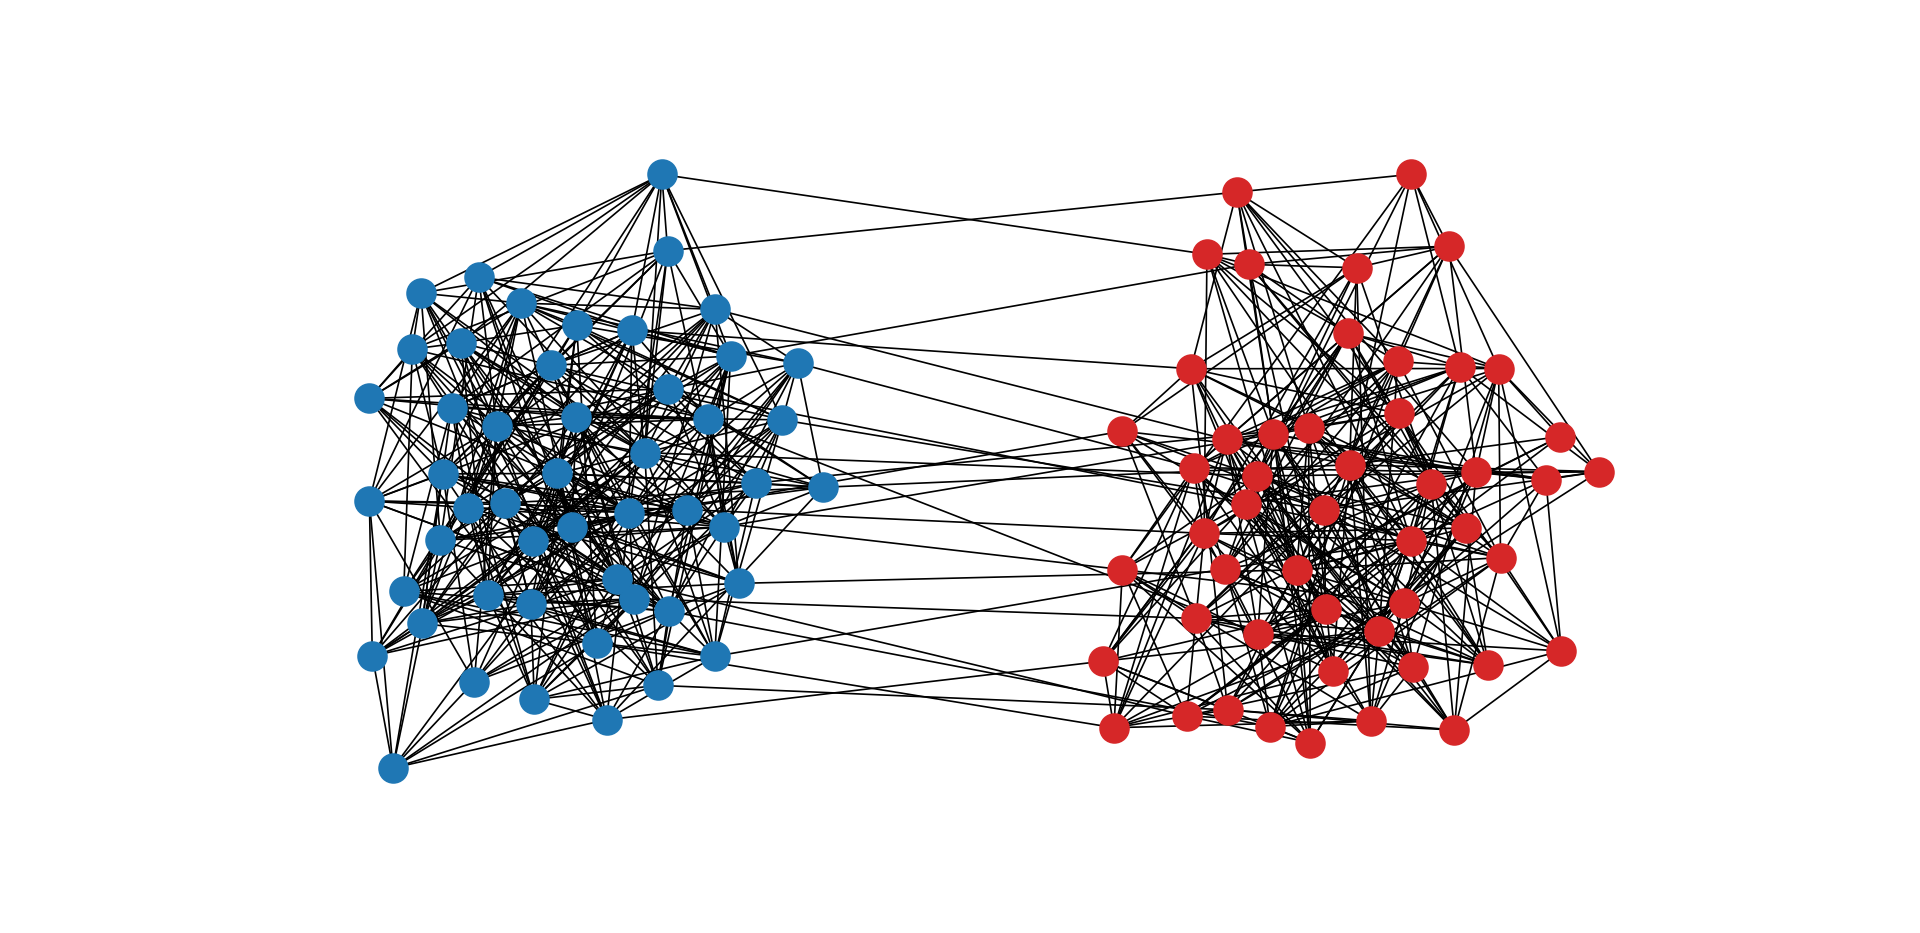
\includegraphics[width=\textwidth]{two-clustering}
\caption{Two ER graphs joined by a few edges.}
\end{subfigure}
\hfill
\begin{subfigure}[b]{0.49\textwidth}
\centering
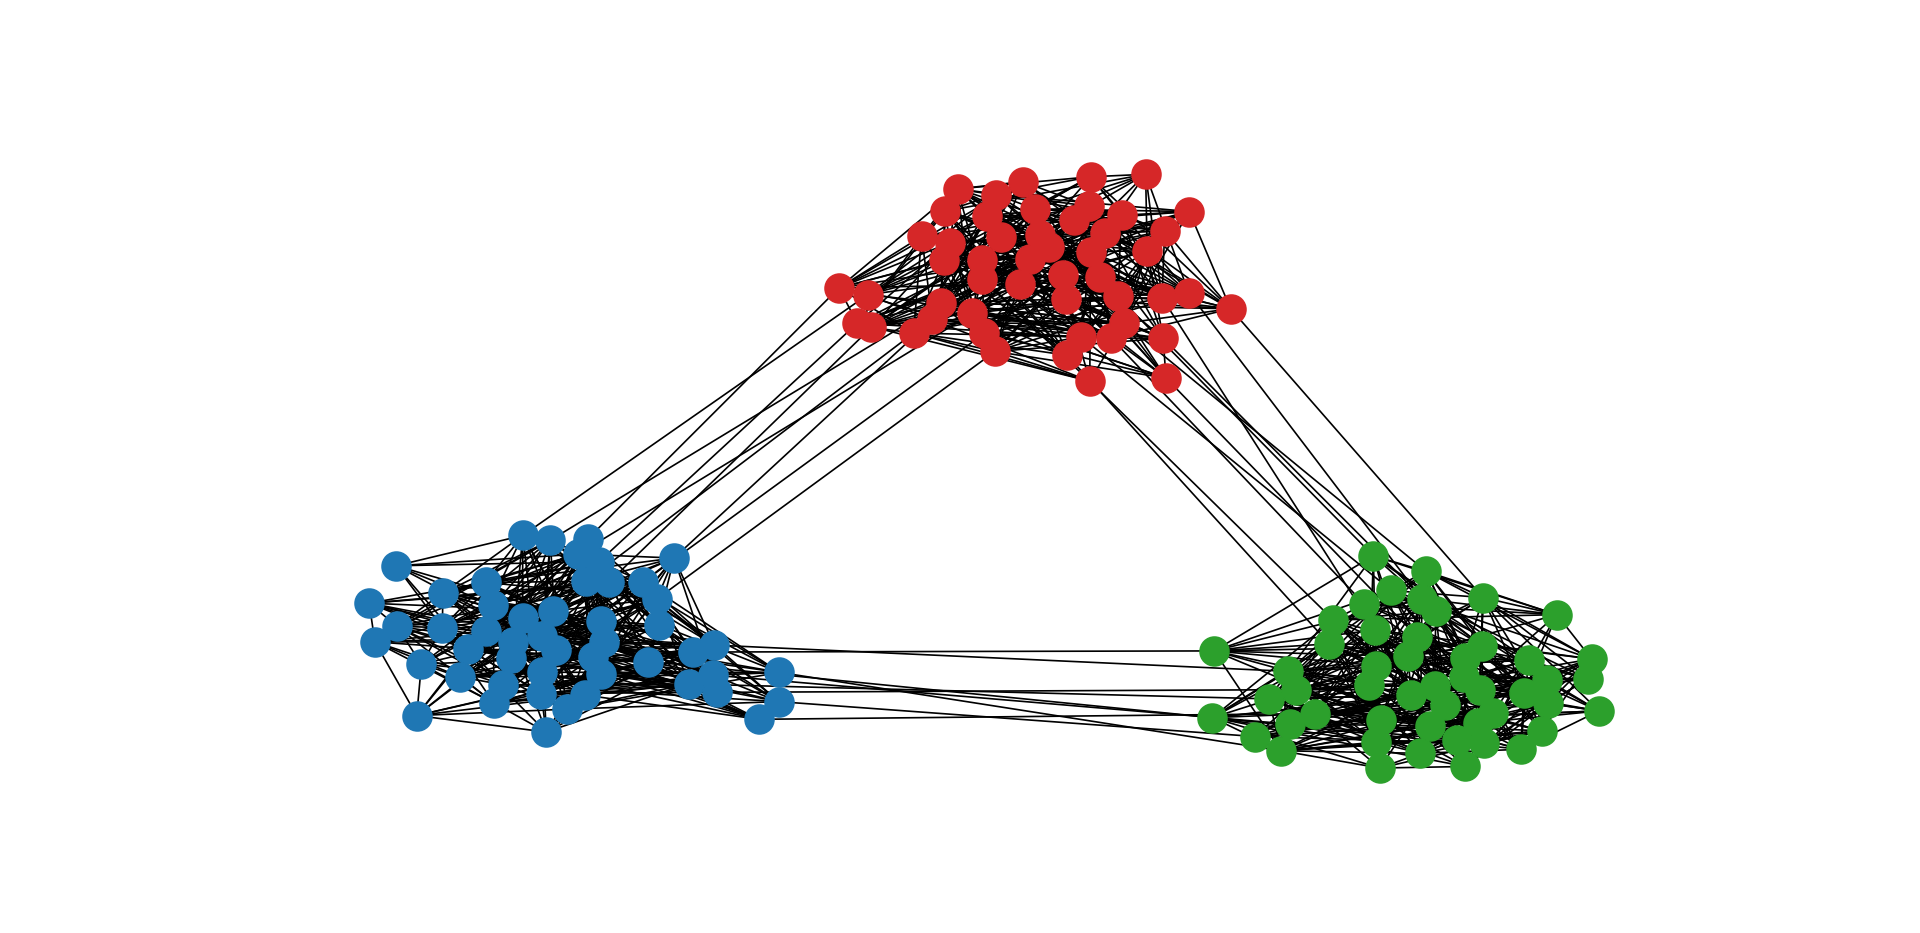
\includegraphics[width=\textwidth]{three-clustering}
\caption{Three ER graphs joined by a few edges.}
\end{subfigure}

\begin{subfigure}[b]{0.49\textwidth}
\centering
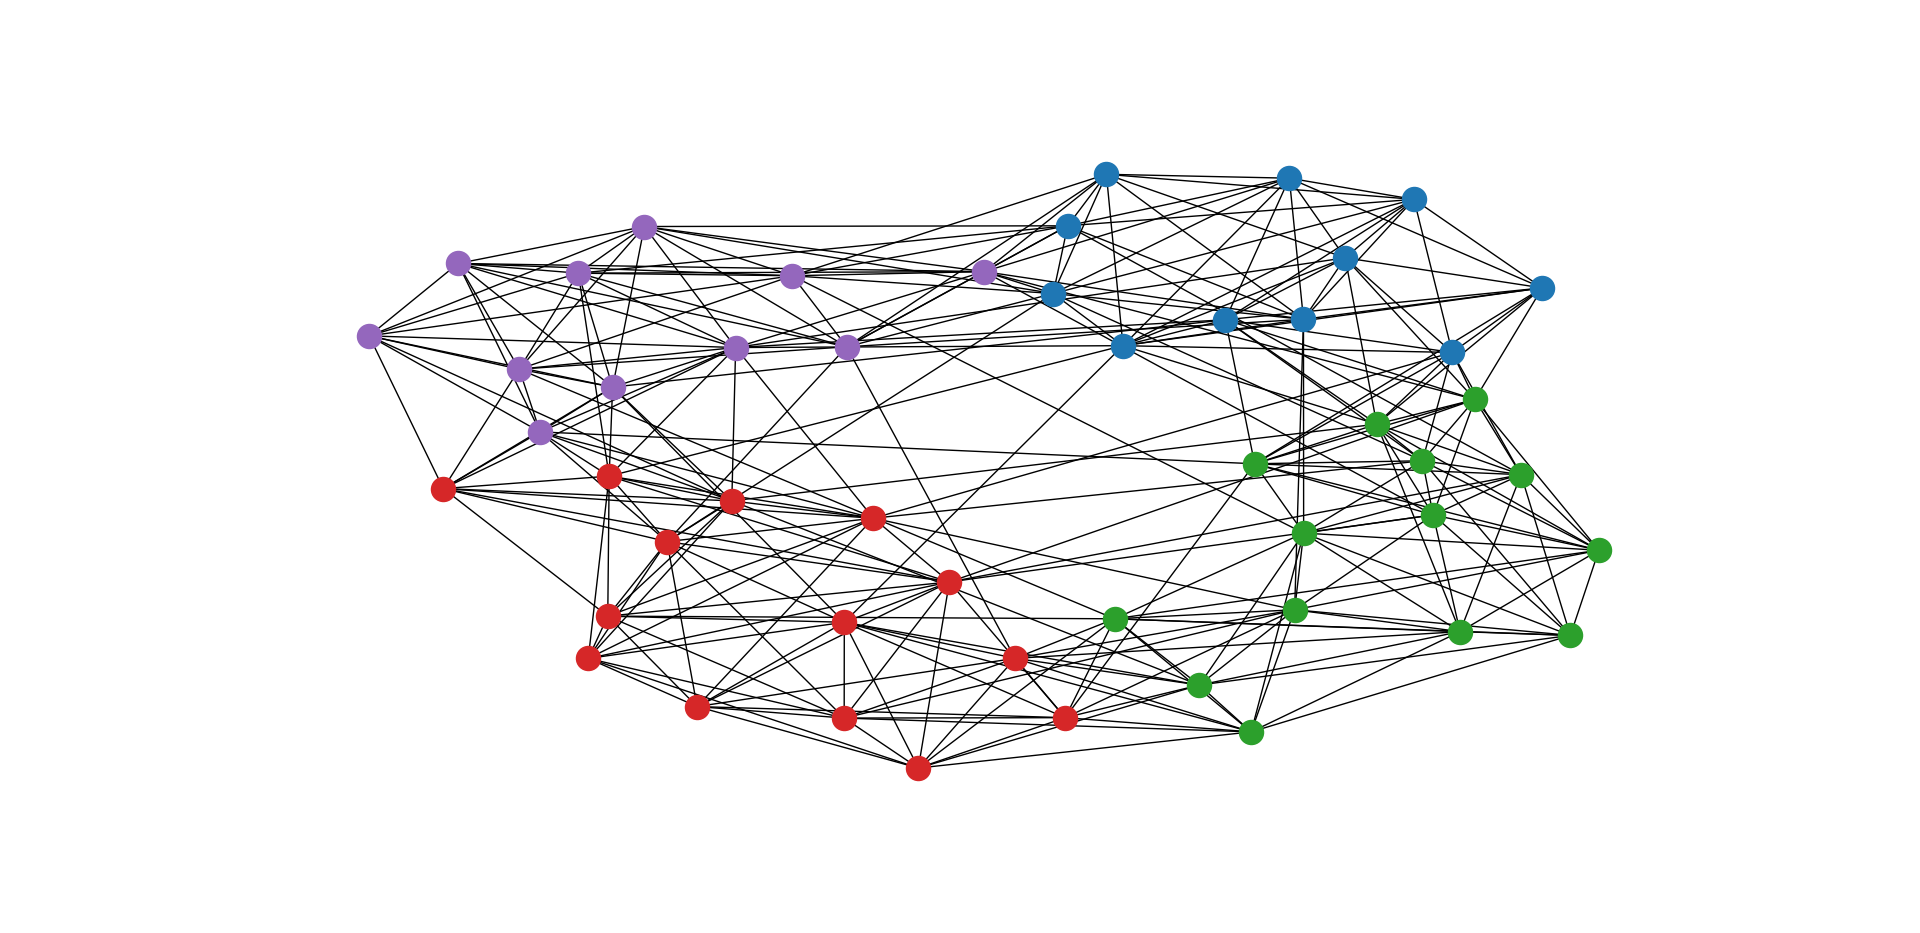
\includegraphics[width=\textwidth]{newman-watts-strogatz}
\caption{Newman–Watts–Strogatz graph with $n = 50, k = 10, p = 0.2$.}
\end{subfigure}
\hfill
\begin{subfigure}[b]{0.49\textwidth}
\centering
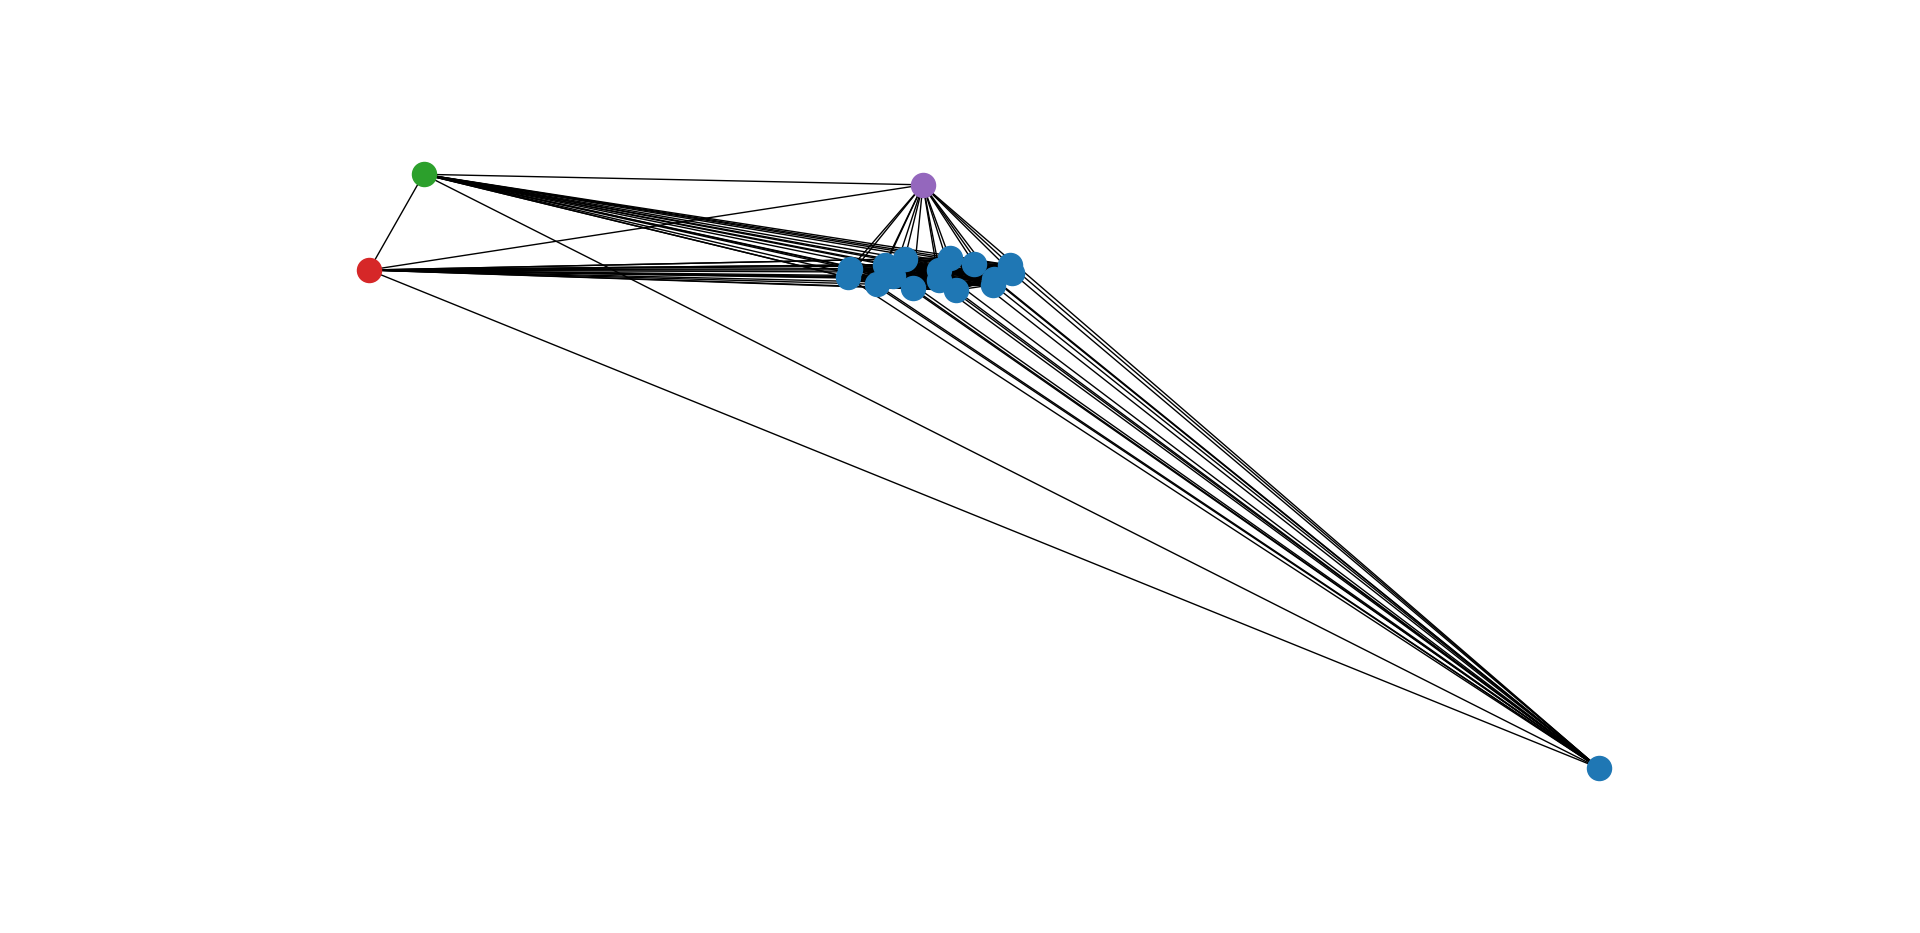
\includegraphics[width=\textwidth]{spectral-gap}
\caption{Graph created via Algorithm \ref{inverse-graph-construction}. 4 small eigenvalues, 16 large eigenvalues.}
\end{subfigure}
\caption{Examples of spectral clustering.}\label{spectral-clustering-algo-results}
\end{figure}

\subsubsection{Efficiency}

The popularity of spectral clustering comes from its efficiency. While general linear systems of the form $Ax = b$ can currently be solved for a vector $x$ in time $O(n^{2.37286})$ \cite{fast-matsolve}, it is possible to solve systems involving the Laplacian matix much faster. Laplacian matrices are examples of \emph{symmetric diagonally dominant} (SDD) matrices, in which each diagonal element is greater than or equal to the sum of the corresponding row. Spielman and Teng \cite{fast-laplacian} provide an $\varepsilon$-approximate method to solve SDD systems with $m$ non-zero entries in time
\[
m \log^{O(1)}(m) + O\left(\left[\log \frac{\lambda_n}{\varepsilon \lambda_2} \right] \left[m + n 2^{O(\sqrt{\log n \log \log n}}) \right] \right),
\]
which (with an appropriate degree of eye-squinting) is said to be `nearly-linear time'. This can be used to produce a set of orthonormal eigenvectors as required by Algorithm \ref{spectral-clustering-algo}. We refer the reader to \cite{vishnoi} for a detailed exposition of fast Laplacian solvers.

\subsection{Image segmentation}

Spectral clustering has been used successfully in computer vision. The first such application was proposed by Shi and Malik \cite{shimalik} to perform image segmentation, in which the goal is to split an image up into multiple segments as would be perceived by a human. The basic idea is as follows:

First, compute a similarity graph $G = (V, E, w)$ where each vertex corresponds to one pixel. For $x, y \in V$ weights are given by
\begin{equation}\label{image-segmentation-weights}
w(x, y) = \begin{cases}
0 \hspace{1em}\text{if } \|X(i) - X(j)\| > r \\
\exp\left(-\|F(i) - F(j)\|^2\right) \cdot \exp\left(-\|X(i) - X(j)\|^2 \right) \text{ otherwise}
\end{cases}
\end{equation}
where $F(i) \in \R$ and $X(i) \in \R^2$ give the brightness and cartesian coordinates of pixel $i$ respectively, and $r \in \R$ is some particular threshold which helps to limit the amount of computation required. Then, spectral clustering is performed on this graph as usual to obtain $k$ clusters of pixels.

\medskip

Shi and Malik propose this scheme in \cite{shimalik}. They instead choose to compute eigenvectors of a similar matrix $\L' = I - D^{-1}W$, which are the differ to the eigenvectors of $\L$ by a factor of $D^{1/2}$. An example input image and the corresponding eigenvectors of $\L'$ are shown in Figure \ref{shi-malik-result}.

\begin{figure}
\centering
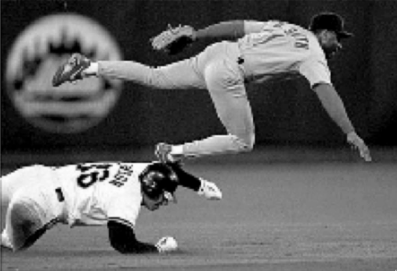
\includegraphics[width=0.6\textwidth]{shi-malik-input} \\
\vspace{0.5cm}
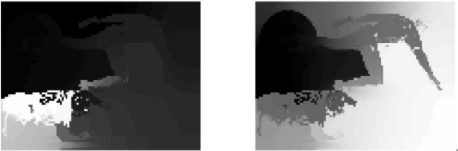
\includegraphics[width=0.8\textwidth]{shi-malik-eigenvectors}
\caption{Input (top), first and second eigenvectors (left and right). Reproduced from \cite{shimalik}.}\label{shi-malik-result}
\end{figure}

\medskip

One may ask: if $k$-means clustering is used during the spectral clustering algorithm, why not apply $k$-means clustering directly with the distance function given by \eqref{image-segmentation-weights}? The answer, provided by Ng, Jordan and Weiss \cite{ngjordanweiss}, is that $k$-means clustering performs poorly when clusters do not form convex regions in the space of the embedding. This is demonstrated by Figure \ref{ngjordanweiss-image-spec}, which shows a set of points in $\R^2$ being clustered either directly by $k$-means, or by constructing a graph in which each point is joined to each of its 10 nearest neighbours with weight proportional to the distance, and then performing spectral clustering.

\begin{figure}
\centering
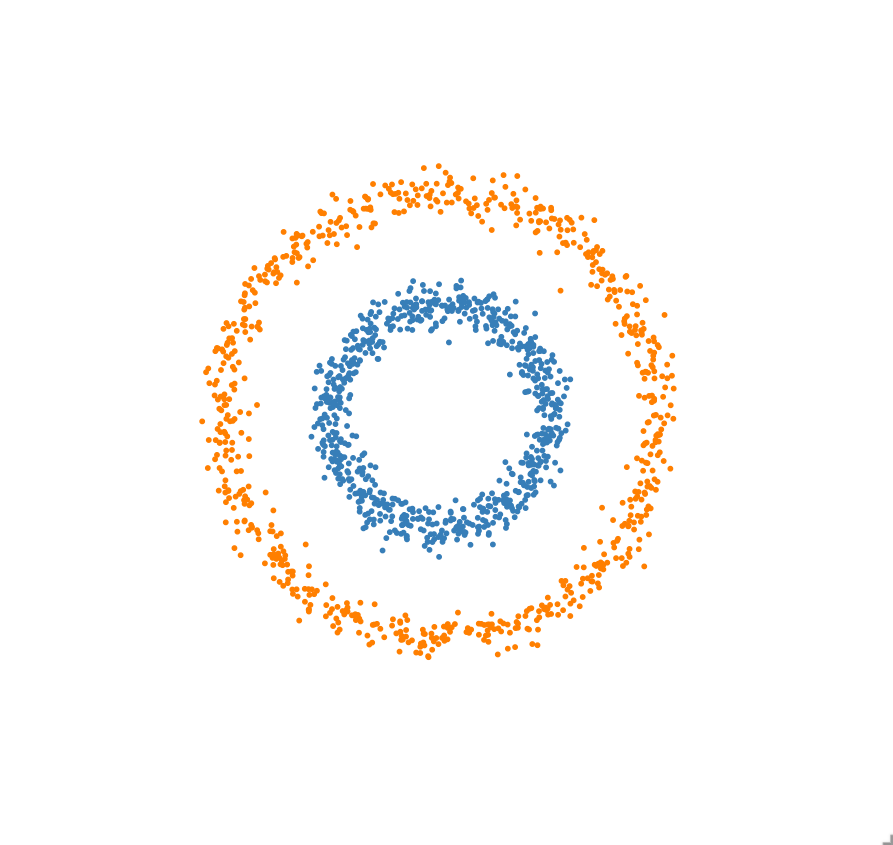
\includegraphics[width=0.4\textwidth]{scikit-spectral-clustering}
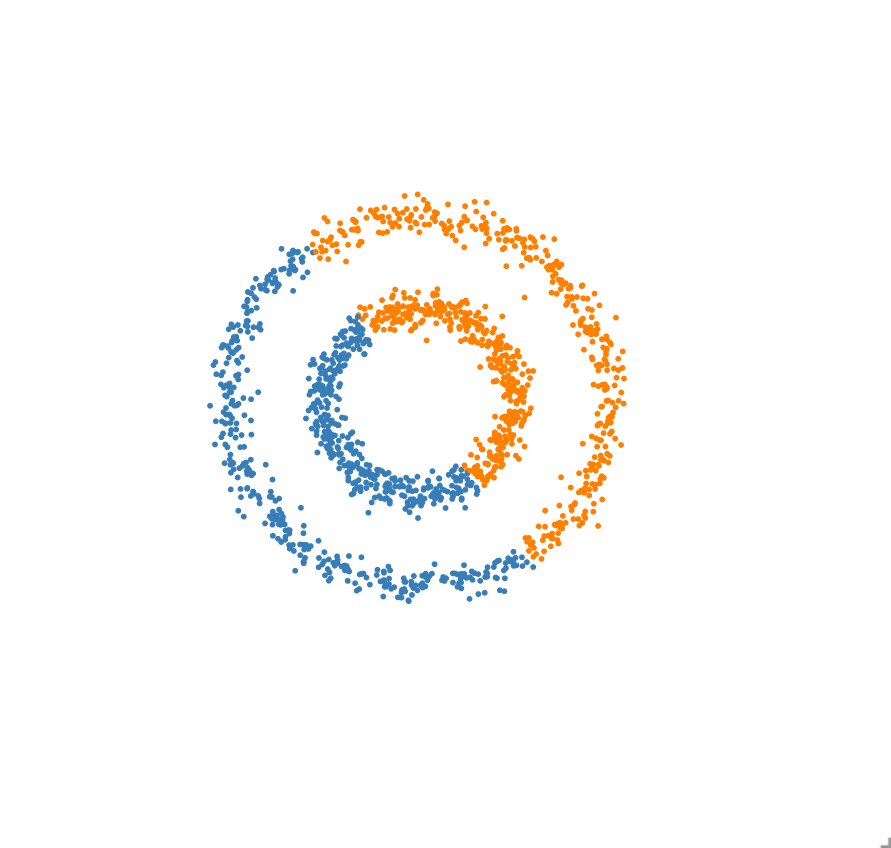
\includegraphics[width=0.4\textwidth]{scikit-kmeans}
\caption{Spectral clustering (left), $k$-means clustering (right).}\label{ngjordanweiss-image-spec}
\end{figure}

\subsection{VLSI design}

More generally, graph clustering may be used to design efficient divide-and-conquer algorithms where the runtime of the `conquer' step is highly dependent on the number of edges.

For example, spectral clustering has been used successfully in Very Large Scale Integration (VLSI) design. VLSI is the process by which huge numbers of transistors are combined to produce integrated circuits. Since many design tools and algorithms are not practical to be run on the millions or billions of components at once, \emph{circuit partitioning} may be employed to decompose the overall design into a few components which can be analysed and optimised independently, with few wires between them. See \cite{vlsi} for a survey of such techniques, and \cite{vlsi-spectral} for a particular example of spectral clustering applied in this area.

Some modifications must be performed to model circuits effectively. Notably, the circuit is represented as a \emph{hypergraph}, since a single wire may join multiple components. This is a particularly crucial fact to capture in the partitioning step, since the number (and weight) of edges leaving a cluster is the exact thing which graph clustering attempts to minimise.

\subsection{Vertex centrality}

One final application we study is the identification of important or `central' vertices in a graph. For example, consider a graph representation of a social network. An intelligent advertiser may choose the most influential people in the network to promote a product, in the hopes that they will spread it to the largest possible number of their peers, and so on.

\medskip

One obvious metric for this is the vertex degree, which for a vertex $x \in V$ is given by $w(x)$. However this is a poor estimate when the neighbours of $x$ have low degree themselves, so we need to capture some global information about the position of the vertex in the graph beyond the degree.

Instead we may desire a metric for which $x$'s importance is the sum of the importance of its neighbours (weighted by the value on the edge), e.g some vector $f \in \R^n$ and $\lambda \in \R$ such that
\begin{equation}\label{eigenvector-centrality-eqn}
f(x) = \frac{1}{\lambda} \sum_{\substack{y \\ y \sim x}} w(x, y) f(y) = \frac{1}{\lambda} \sum_{y \in V} W_{xy} \cdot f(y)
\end{equation}
which can be rewritten as the eigenvector problem $Wf = \lambda f$. The Perron-Frobenius theorem tells us that $f$ corresponds to the unique greatest real eigenvalue of $W$, and moreover that $f$ has strictly positive entries.

\medskip

This eigenvector can be computed efficiently using the power iteration method (Algorithm \ref{power-iteration}). At each iteration, the vector is normalised to retain precision during computation (otherwise the components will become too large or too small, and accuracy will suffer).

\begin{algorithm}
\caption{Power iteration}\label{power-iteration}
\Fn{\text{\upshape centrality}$(G)$}{
    \KwIn{Graph $G$ with weight matrix $W$}
    \KwOut{$f \in \R^n$ giving the eigenvector centrality of each vertex}
    \DontPrintSemicolon
    \BlankLine
    $x \gets $ uniform random vector in $\R^n$\;
    $\mathrm{change} \gets \infty$\;
    \While{$\mathrm{change} > \varepsilon$}{
        $x' \gets \frac{Wx}{\|Wx\|}$\;
        $\mathrm{change} \gets \|x' - x\|$\;
        $x \gets x'$\;
    }
    \Return{$x$}\;
}
\end{algorithm}

Google's search engine is based on a similar centrality measure called \textbf{PageRank}. The basic idea is to represent the web as a unweighted directed graph $G = (V, E)$ where the vertices correspond to webpages and the edges correspond to links between pages. When a user types a query into Google, the search engine will return a set of matching results ordered by their PageRank (and nowadays, countless other factors), under the assumption that users will want to see the most important or `central' webpages first.

\medskip

The computation of PageRank can be expressed as an eigenvector problem similar to \eqref{eigenvector-centrality-eqn}, and is performed via a power iteration method. For this reason, Bryan and Leise \cite{google-eigenvector} describe PageRank as the `\$25,000,000,000 eigenvector'. It is safe to say that the applications of spectral graph theory are numerous and profound.
\bibliographystyle{unsrt}
\bibliography{references}

\end{document}
